\section{Integration}

  \subsection{Construction of the Riemann Integral}

    We shall first define the integral using the familiar notation of Riemann sums. 

    \begin{definition}[Partitions with Distinguished Points]
      A \textbf{partition} $P$ of a closed interval $[a, b]$, $a < b$, is a finite system of points $x_0, \ldots, x_n$ of the interval such that
      \[a = x_0 < x_1 < x_2 < \ldots < x_n = b\]
      The intervals $[x_{i-1}, x_i]$, $i = 1, 2, \ldots, n$, are called the \textbf{intervals} of the partition $P$. The largest of the lengths of the intervals of the partition $P$, denoted $\lambda(P)$, is called the \textbf{mesh} of the partition. 

      A \textbf{partition with distinguished points} $(P, \xi)$ on the closed interval $[a, b]$ is a partition $P$ of $[a,b]$ along with the set of $n$ points 
      \[\xi_1 \in [x_0, x_1], \xi_2 \in [x_1, x_2], \ldots, \xi_n \in [x_{n-1}, x_n]\]
      The $n$-tuple of $\xi_i$'s is denoted by the single letter $\xi$
      \[\xi = (\xi_1, \xi_2, \ldots, \xi_n)\]
    \end{definition}

    This naturally leads to the following construction. 

    \begin{definition}[Riemann Sums]
      If a function $f$ is defined on a closed interval $[a, b]$ and $(P, \xi)$ is a partition with distinguished points on this closed interval, the sum
      \[\sigma(f; P, \xi) \equiv \sum_{i=1}^n f(\xi_i)\, \Delta x_i, \text{ where } \Delta x_i = x_i - x_{i-1},\]
      is the \textbf{Riemann sum} of the function $f$ corresponding to the partition $(P, \xi)$ with distinguished points on $[a, b]$. 
      \begin{center}
          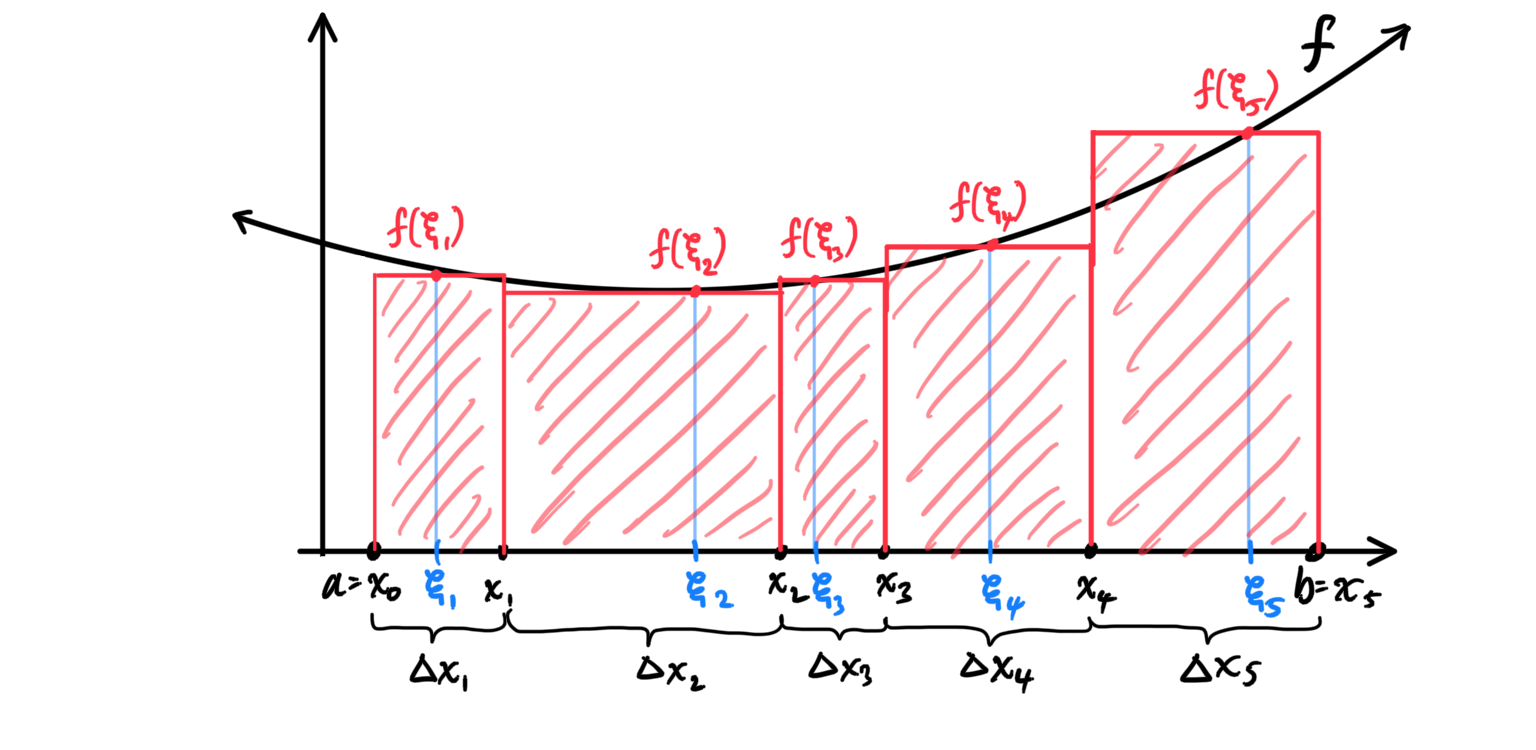
\includegraphics[scale=0.25]{img/Riemann_Sum_with_Partitions_Points.PNG}
      \end{center}
      Thus, when a function $f$ is fixed, the Riemann sum $\sigma (f; P, \xi)$ is a mapping that takes in a partition with distinguished points $p = (P, \xi)$ on the closed interval $[a, b]$ and outputs a number representing the total area of the Riemann sums. That is, for a fixed $f$ and some input $p = (P, \xi)$, we can define the function 
      \[\Phi: \mathcal{P} \longrightarrow \mathbb{R}, \;\;\; \Phi(p) \equiv \sigma(f; p) \equiv \sigma(f; (P, \xi))\]
      that takes in a partition with distinguished points on $[a,b]$ and outputs the corresponding Riemann sum for that fixed $f$. 
    \end{definition}

    \begin{definition}[Riemann Integral]
      The number $\int_a^b f(x)\,dx$ is the \textbf{Riemann integral} of the function $f$ on the closed interval $[a, b]$ if for every $\epsilon>0$ there exists a $\delta>0$ such that
      \[\Bigg| \int_a^b f(x)\,dx - \sum_{i=1}^n f(\xi_i) \Delta x_i \Bigg| < \epsilon\]
      for any partition $(P, \xi)$ with distinguished points on $[a, b]$ whose mesh $\lambda(P)$ is less than $\delta$. We can view this as a limit where $n \rightarrow \infty$, but there is a problem since we can increase the partition within different subsets of $[a,b]$, leading to multiple values of convergence. 
      \begin{center}
          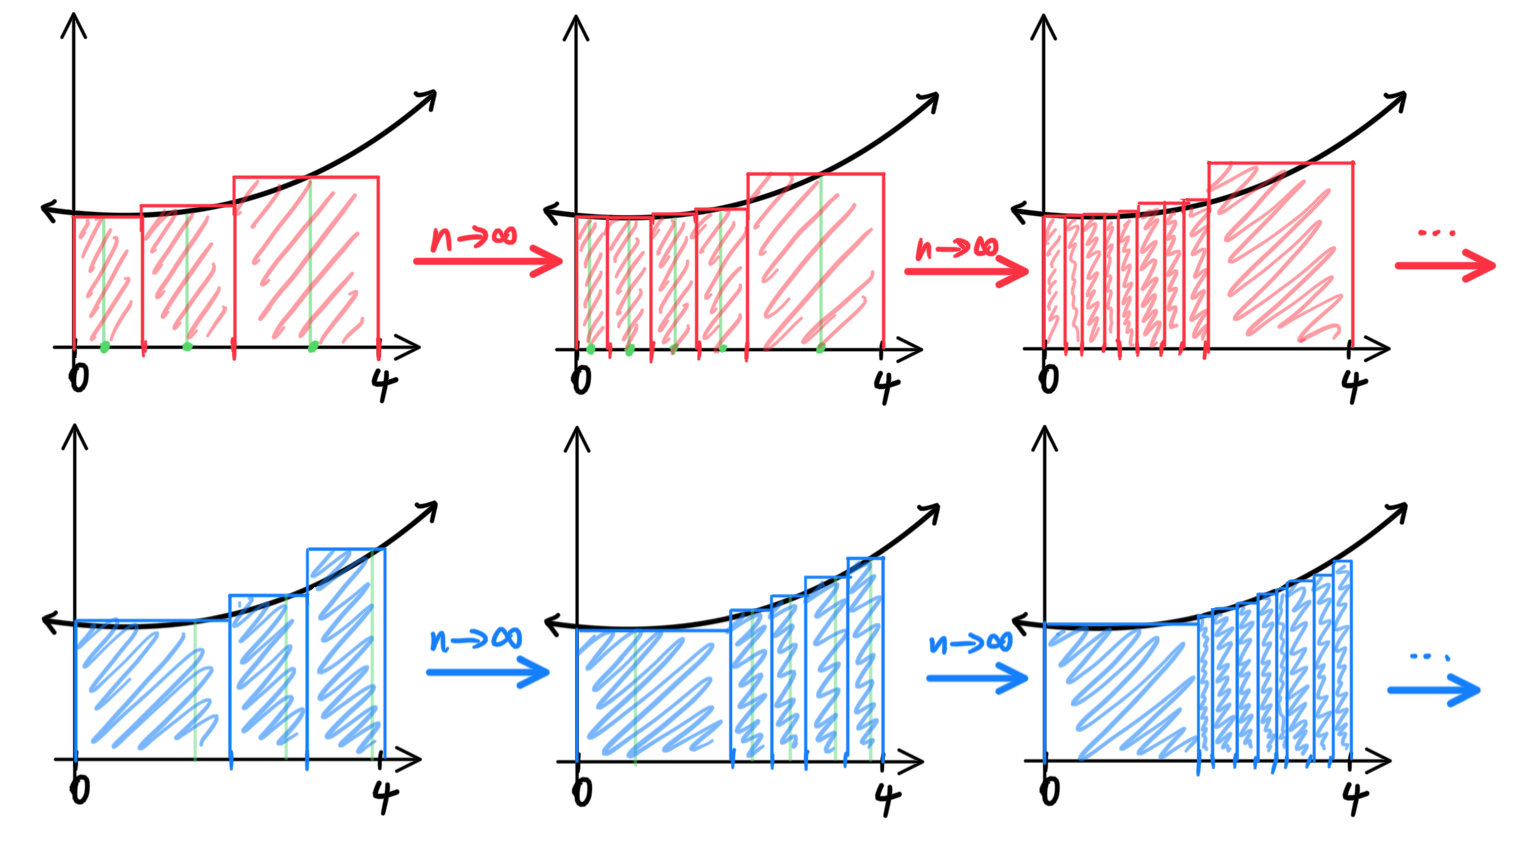
\includegraphics[scale=0.28]{img/Riemann_Integral_Converging_onto_2_Numbers.PNG}
      \end{center}
      Rather, we can set the mesh $\lambda(P)$ to approach $0$, which would take care of the problems. We can visualize this by imagining the lengths of the rectangles converging "uniformly."
      \begin{center}
          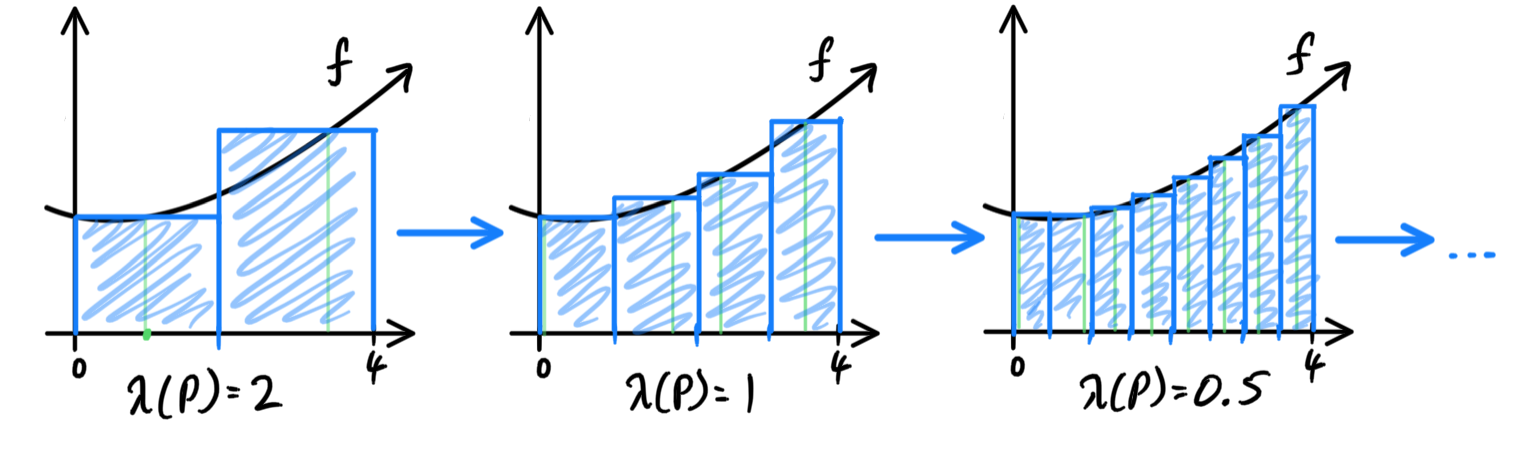
\includegraphics[scale=0.28]{img/Riemann_Integral_Limit_Mesh_goes_to_0.PNG}
      \end{center}
      Therefore, we can culminate by defining the Riemann integral of $f(x)$ over $[a,b]$ as 
      \[\int_a^b f(x)\,dx \equiv \lim_{\lambda(P) \rightarrow 0} \sum_{i=1}^n f(\xi_i) \lambda x_i\]
    \end{definition}

  \subsubsection{Conditions for Integrability}

    \begin{definition}[Riemann Integrable Functions]
      A function $f$ is \textbf{Riemann integrable} on the closed interval $[a, b]$ if 
      \[\int_a^b f(x)\,dx \equiv \lim_{\lambda(P) \rightarrow 0} \sum_{i=1}^n f(\xi_i) \lambda x_i\]
      is defined, i.e. if the limit of the right-hand side of Riemann sums exists as $\lambda(P) \rightarrow 0$ (that is, the Riemann integral of $f$ is defined). 

      Furthermore, the set of Riemann-integrable functions on a closed interval $[a, b]$ is denoted $\mathcal{R}[a,b]$. 
    \end{definition}

    Remember that the Riemann integral, as complicated as the formula is, is still a limit of a function. That means that we can apply the Cauchy criterion to it to determine convergence. 

    \begin{lemma}[Cauchy Criterion on Existence of Riemann Integral]
      Given a function $f$, the integral of $f$ over $[a, b]$, defined
      \[\int_a^b f(x)\,dx \equiv \lim_{\lambda(P) \rightarrow 0} \sum_{i=1}^n f(\xi_i) \lambda x_i\]
      exists if and only if for every $\epsilon>0$, there exists a $\delta>0$ such that 
      \[\big| \sigma(f; P^\prime, \xi^\prime) - \sigma(f; P^{\prime\prime}, \xi^{\prime\prime} \big| < \epsilon\]
      or, what is the same, 
      \[\Bigg| \sum_{i=1}^{n^\prime} f(\xi_i^\prime) \Delta x_i^\prime - \sum_{i=1}^{n^{\prime\prime}} f^(\xi_i^{\prime\prime}) \Delta x_i^{\prime\prime} \Bigg| < \epsilon\]
      for any partitions $(P^\prime, \xi^\prime)$ and $(P^{\prime\prime}, \xi^{\prime\prime})$ with distinguished points on the interval $[a, b]$ with
      \[\lambda(P^\prime), \lambda(P^{\prime\prime}) < \delta\]
      In words, this means that for any $\epsilon>0$ that we choose, there always exists a $\delta>0$ such that \textbf{any} two Riemann sums with mesh size \textbf{both} smaller than $\delta$ will have an error difference of less than $\epsilon$. \begin{center}
          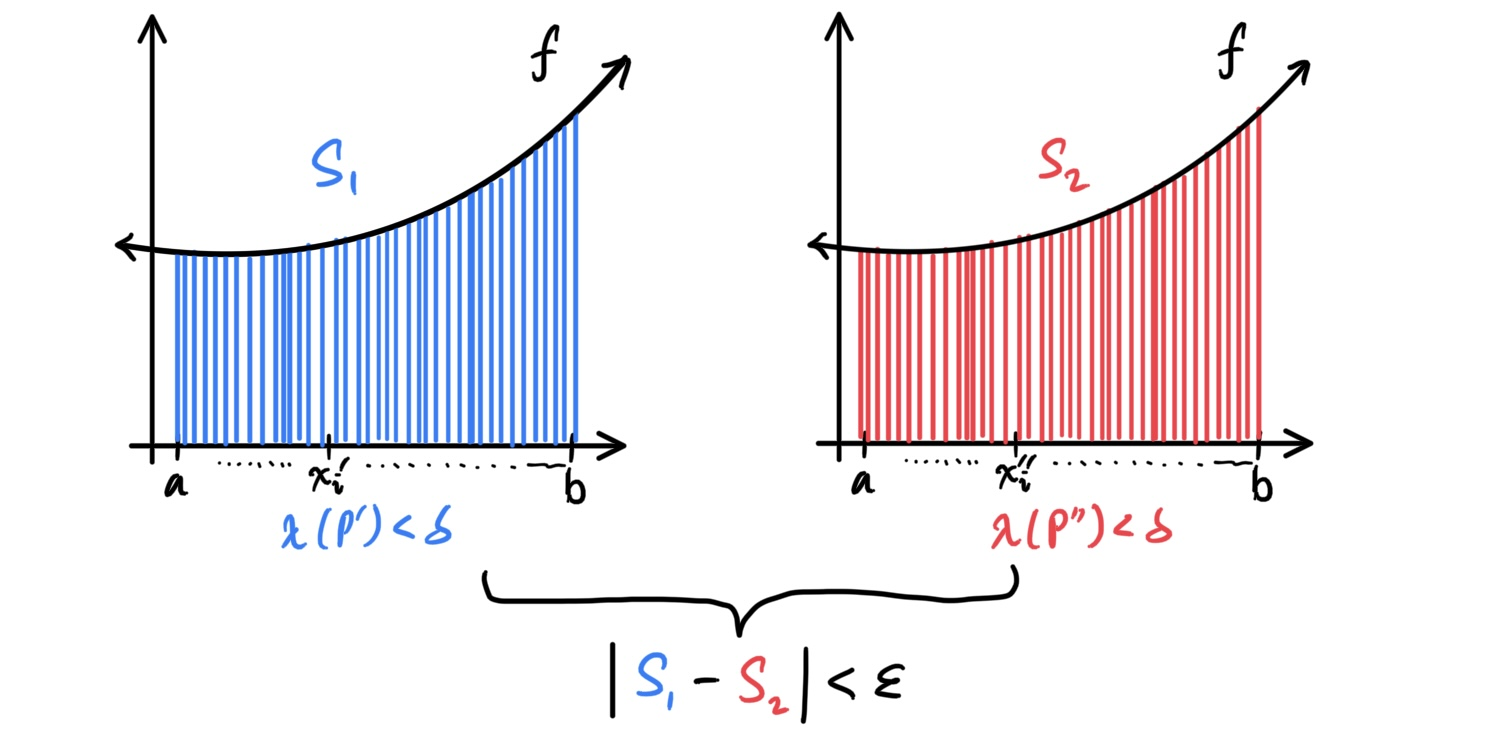
\includegraphics[scale=0.25]{img/Cauchy_Criterion_of_Riemann_Integral.jpg}
      \end{center}
    \end{lemma}

    \begin{theorem}[Necessary Condition for Integrability]
    A necessary condition for $f$ defined on a closed interval $[a, b]$ to be Riemann integrable on $[a, b]$ is that $f$ be bounded on $[a, b]$. That is, 
    \[f \in \mathcal{R}[a, b] \implies f \text{ is bounded on } [a, b]\]
    We can clearly see the necessity of $f$ being bounded by looking at the contrapositive of the following statement. 
    \end{theorem}

    \begin{theorem}[Refinement]
    Given a partition $P$ on interval $[a, b]$, recall that we have points $x_0, \ldots, x_n$ such that
    \[a = x_0 < x_1 < \ldots < x_n = b\]
    Here we introduce new notation: 
    \begin{enumerate}
      \item $\Delta_i$ denotes the interval $[x_{i-1}, x_i]$
      \item $\Delta x_i$ denotes the difference $x_i - x_{i-1}$, i.e. the length of $\Delta_i$
    \end{enumerate}
    If a partition $\Tilde{P}$ of the closed interval $[a, b]$ is obtained from the partition $P$ by the addition of new points to $P$, we call $\Tilde{P}$ a \textbf{refinement} of $P$. 

    When a refinement $\Tilde{P}$ of a partition $P$ is constructed, some (perhaps all) of the closed intervals $\Delta_i = [x_{i-1}, x_i]$ of the partition $P$ themselves undergo partitioning. 
    \[x_{i-1} = x_{i0} < x_{i1} < \ldots < x_{in_i} = x_i\]
    In that connection, it will be useful to label to points of $\Tilde{P}$ by double indices, where in the notation $x_{ij}$ the first index $i$ means that 
    \[x_{ij} \in \Delta_i = [x_{i-1}, x_i]\]
    and the second index $j$ is the ordinal number of the point on the closed interval $\Delta_i = [x_{i-1}, x_i]$. Therefore, it is natural to set the notations
    \begin{enumerate}
      \item $\Delta_{ij} = [x_{i j-1}, x_{ij}]$
      \item $\Delta x_{ij} = x_{ij} - x_{ij-1}$
    \end{enumerate}
    This means that 
    \[\Delta x_i = \Delta x_{i1} + \Delta x_{i2} + \ldots + \Delta x_{in_i}\]
    which can be visualized below
    \begin{center}
      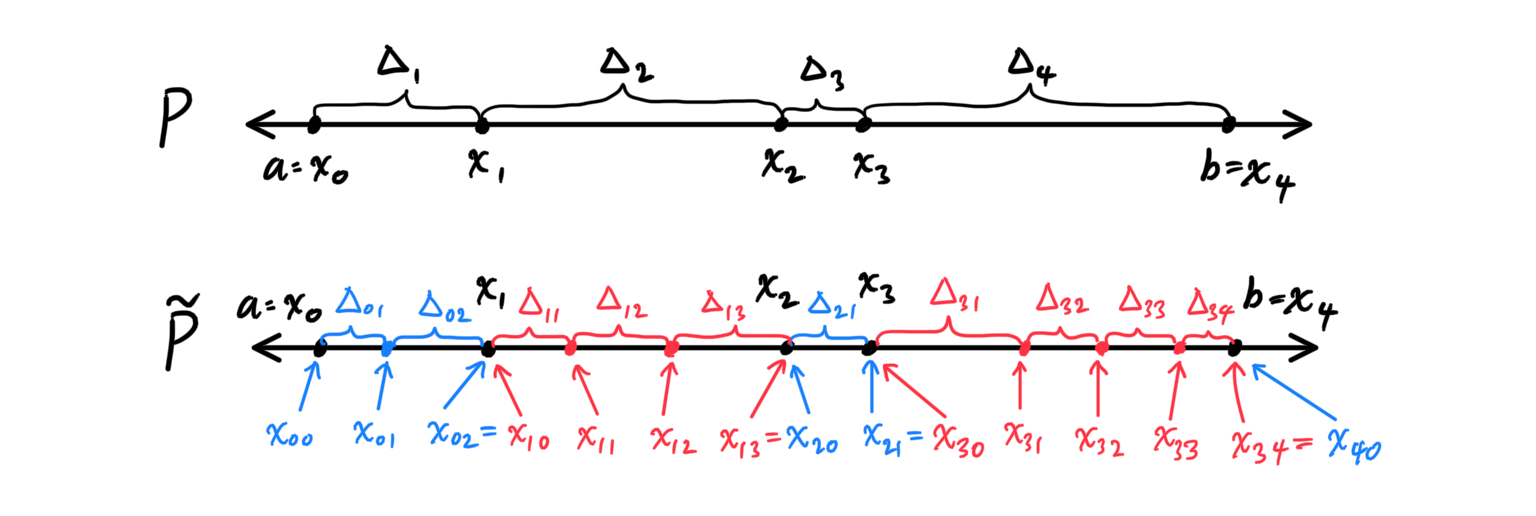
\includegraphics[scale=0.25]{img/Refinement_Definition_Analysis.PNG}
    \end{center}
    \end{theorem}

    \begin{example}[Union of Partitions as a Refinement]
    For some interval $[a, b]$, given partitions $P^\prime$ ($a = x_0 < \ldots < x_n = b$) and $P^{\prime\prime}$ ($a = y_0 < \ldots < y_n = b$), the union of the two partitions $\Tilde{P} = P^\prime \cup P^{\prime\prime}$ is a refinement of both $P^\prime$ and $P^{\prime\prime}$. 
    \begin{center}
        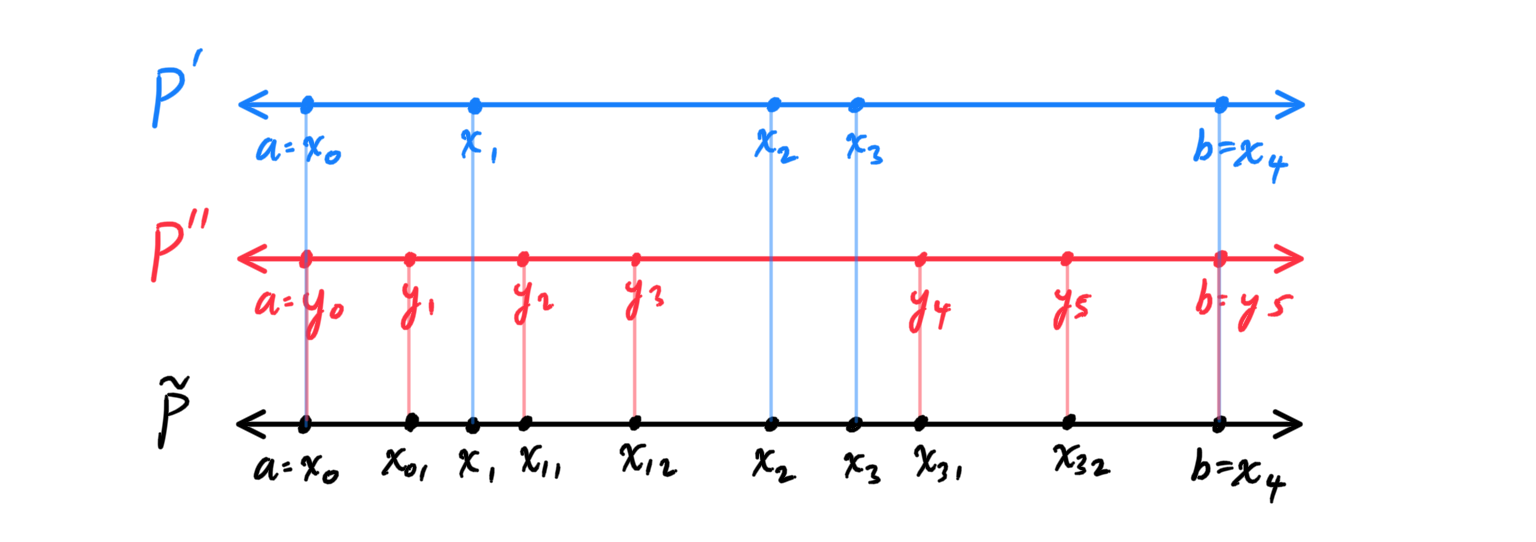
\includegraphics[scale=0.25]{img/Refinement_as_Union_of_Partitions.PNG}
    \end{center}
    \end{example}
    
    Recall that $\omega(f; E)$ denotes the oscillation of the function $f$ on the set $E$; that is, 
    \[\omega(f; E) \equiv \sup_{x^\prime, x^{\prime\prime} \in E} \big| f(x^\prime) - f(x^{\prime\prime})\big|\]
    In particular, $\omega(f; \Delta_i)$ is the oscillation of $f$ on the closed interval $\Delta_i$. 

    \begin{theorem}[Sufficient Condition for Integrability]
    Let $f$ be a bounded on a closed interval $[a, b]$ such that for every $\epsilon > 0$ there exists a number $\delta>0$ such that
    \[\sum_{i=1}^n \omega(f; \Delta_i) \Delta x_i < \epsilon\]
    for any partition $P$ of $[a, b]$ with mesh $\lambda(P) < \delta$. This is equivalent to saying that
    \[\lim_{\lambda(P) \rightarrow 0} \sum_{i = 1}^n \omega (f; \Delta_i) \, \Delta x_i = 0\]
    Then, $f$ is integrable. We can visualize
    \[\sum_{i=1}^n \omega(f; \Delta_i) \Delta x_i\]
    as the following sum of rectangles below. 
    \begin{center}
        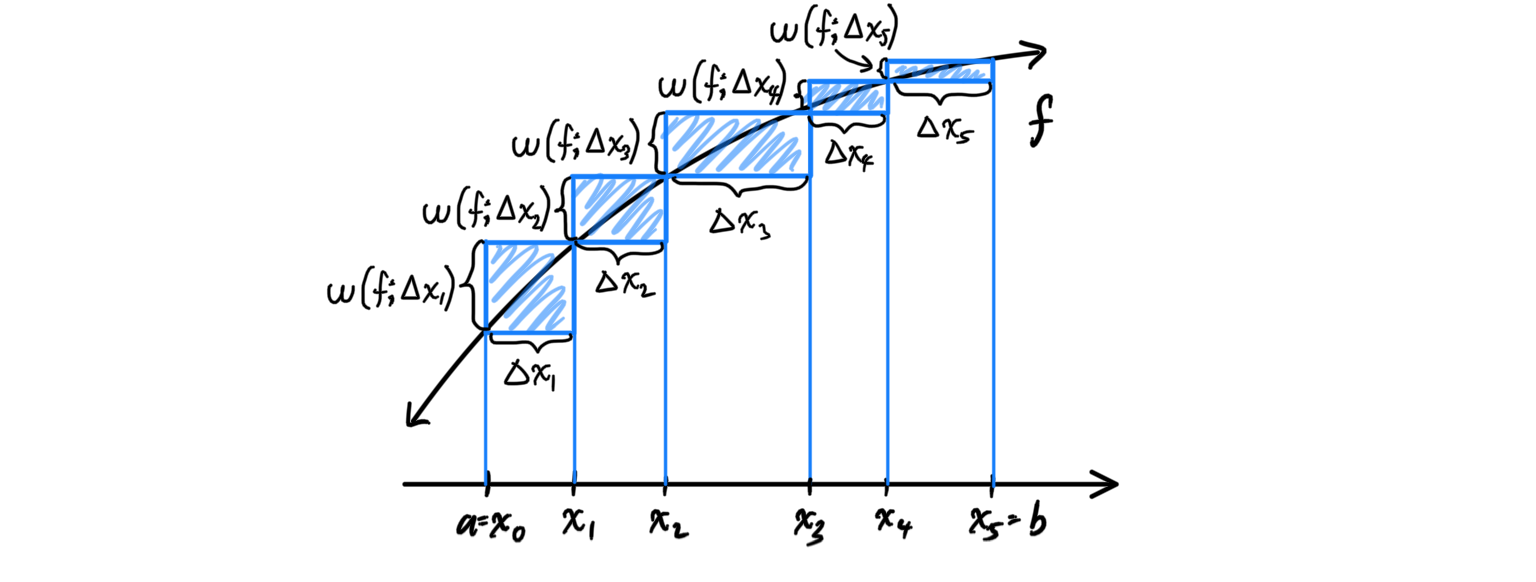
\includegraphics[scale=0.25]{img/Sufficient_Condition_for_Integrability.PNG}
    \end{center}
    What the theorem states, visually, is that as we make all the rectangles smaller and smaller (by putting a limit on the mesh $\lambda(P)<\delta$), we can make the sum of all these rectangles also arbitrarily small. 
    \end{theorem}

    \begin{corollary}[Integrability of Continuous Functions]
    Every continuous function on a closed interval is integrable on that closed interval. That is, 
    \[f \in C[a, b] \implies f \in \mathcal{R}[a, b]\]
    \end{corollary}

    We can actually make a stronger claim. 

    \begin{corollary}[Integrability of Discontinuous Functions]
    If a bounded function $f$ on a closed interval $[a, b]$ is continuous everywhere except at a finite set of points, then $f \in \mathcal{R}[a, b]$. 
    \end{corollary}

    \begin{corollary}[Integrability of Monotonic Functions]
    A bounded monotonic function on a closed interval is integrable on that interval. 
    \begin{center}
        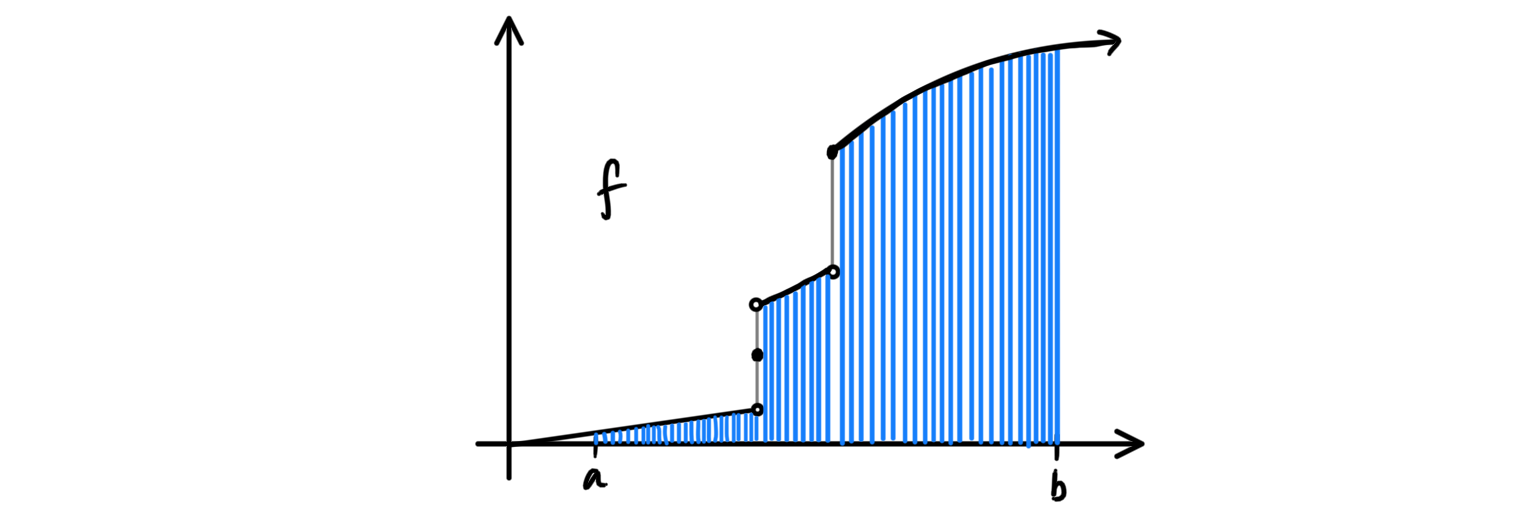
\includegraphics[scale=0.25]{img/Integrability_of_Monotonic_Function.PNG}
    \end{center}
    \end{corollary}

    \begin{definition}[Upper, Lower Riemann Sums]
      Let $f: [a, b] \longrightarrow \mathbb{R}$ be a real-valued function that is defined and bounded on the closed interval $[a, b]$, and let $P$ be a partition of $[a, b]$, and let $\Delta_i$ ($i = 1, 2, \ldots, n$) be the intervals of the partition $P$. Let 
      \begin{align*}
          m_i &= \inf_{x \in \Delta_i} f(x) \\
          M_i &= \sup_{x \in \Delta_i} f(x)
      \end{align*}
      be the infimum and supremum of $f$ over $\Delta x_i$. Then, the sums
      \begin{align*}
          s(f; P) & \equiv \sum_{i = 1}^n m_i \, \Delta x_i \\
          S(f; P) & \equiv \sum_{i=1}^n M_i \, \Delta x_i
      \end{align*}
      are respectively called the \textbf{lower} and \textbf{upper Riemann sums} of the function $f$ on the interval $[a, b]$ corresponding to the partition $P$ of that interval. 

      Given an arbitrary partition $(P, \xi)$ with distinguished points on $[a, b]$, it is clear that
      \[s(f; P) = \inf_{\xi} \sigma(f; P, \xi) \leq \sigma(f; P, \xi) \leq \sup_{\xi} \sigma(f; P, \xi) = S(f; P)\]
    \end{definition}

    \begin{theorem}
    A bounded real-valued function $f: [a, b] \longrightarrow \mathbb{R}$ is Riemann integrable on $[a, b]$ if and only if the following limits exist and are equal to each other. 
    \[\underline{I} \equiv \lim_{\lambda(P) \rightarrow 0} s(f; P) = \lim_{\lambda(P) \rightarrow 0} S(f; P) \equiv \overline{I}\]
    When the relation is true, then the integral is this common value. 
    \[\int_a^b f(x) \,dx = \underline{I} = \overline{I}\]
    \end{theorem}

    Note that this condition of the upper and lower Riemann sums converging to the same value and the condition that 
    \[\lim_{\lambda(P) \rightarrow 0} \sum_{i = 1}^n \omega (f; \Delta_i) \, \Delta x_i = 0\]
    are the same. For we can see that the rectangles visualized from the equation above are the exact same rectangles formed by $S(f; P) - s(f; P)$! 
    \begin{center}
        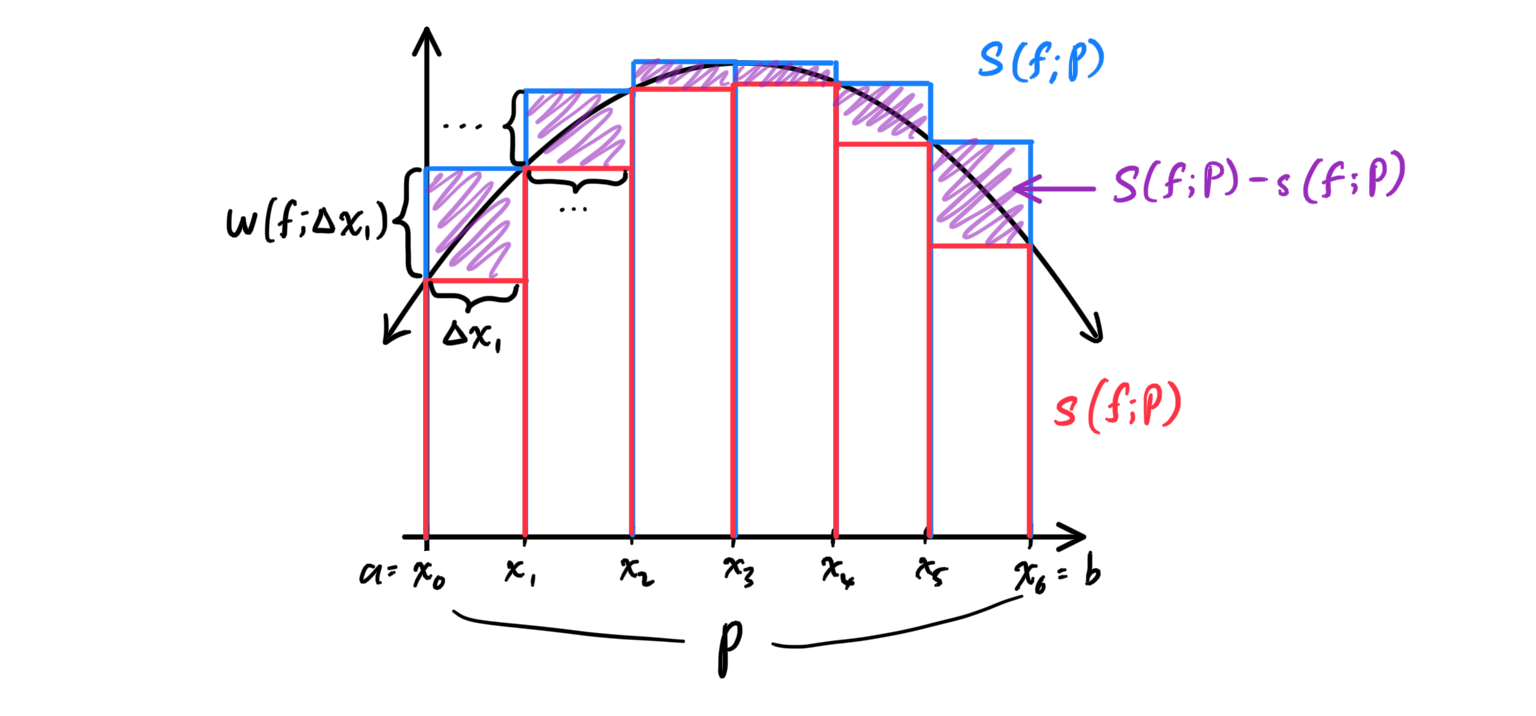
\includegraphics[scale=0.3]{img/Equivalent_Conditions_for_Integrability.PNG}
    \end{center}

    \subsubsection{The Vector Space of Riemann Integrable Functions}

    \begin{theorem}[The Vector Space of Integrable Functions]
    The set of Riemann integrable functions $\mathcal{R}[a, b]$ over closed interval $[a, b]$ is a vector space. That is, given $f, g \in \mathcal{R}[a, b]$ and $\alpha \in \mathbb{R}$, then
    \begin{enumerate}
      \item $(f + g) \in \mathcal{R}[a, b]$ 
      \item $(\alpha f) \in \mathcal{R}[a, b]$
    \end{enumerate}
    Furthermore, 
    \begin{enumerate}
      \item $|f| \in \mathcal{R}[a, b]$
      \item The restriction of $f$ in any $[c, d] \subset [a, b]$, denoted $f \big|_{[c,d]}$, is in $\mathcal{R}[c,d]$
      \item $(f \cdot g) \in \mathcal{R}[a, b]$
    \end{enumerate}
    \end{theorem}
    \begin{proof}

    \end{proof}

    \subsubsection{Lebesgue's Criterion for Riemann Integrability}
    We give Lebesgue's version of an intrinsic description of a Riemann integrable function. 

    \begin{definition}[Measure]
      A set $E \subset \mathbb{R}$ has \textbf{(Lebesgue) measure zero} if for every number $\epsilon > 0$ there exists a covering of the set $E$ be an at most countable system $\{I_k\}$ of intervals, the sum of whose lengths 
      \[\sum_{k=1}^\infty |I_k| \leq \epsilon\]
      This means that the above series summing up the lengths of the intervals is an absolutely convergent series. 
    \end{definition}

    \begin{lemma}
      We can deduce measures of basic sets. 
      \begin{enumerate}
        \item A finite number of points are sets of measure zero. 
        \item The union of a finite or countable number of sets of measure zero is a set of measure zero. \item A subset of a set of measure zero is itself a set of measure zero. 
        \item A closed interval $[a, b]$ with $a<b$ is not a set of measure zero. 
      \end{enumerate}
    \end{lemma}

    \begin{definition}
      If a property holds at all points of a set $X$ except possible the points of a set of measure zero, we say that this property holds \textbf{almost everywhere on $X$} or \textbf{at almost every point of $X$}. 
    \end{definition}

    Now, we can state Lebesgue's criterion for integrability, which nicely summarizes what we have so far. 

    \begin{theorem}[Lebesgue's Criterion for Integrability]
    A function defined on a closed interval is Riemann integrable on that interval if and only if it is bounded and continuous at almost every point. 
    \end{theorem}

    \begin{example}[Non-Integrability of the Dirichlet Function]
    The Dirichlet function
    \[\mathcal{D}(x) \equiv \begin{cases}
    1, & \text{ for } x \in \mathbb{Q} \\
    0, & \text{ for } x \in \mathbb{R} \setminus \mathbb{Q}
    \end{cases}\]
    on the interval $[0,1]$ is not integrable on that interval. We state two different reasons why. 
    \begin{enumerate}
      \item For any partition $P$ of $[0,1]$ we can find in each interval $\Delta_i$ both a rational point $\xi^\prime_i$ and an irrational point $\xi_i^{\prime\prime}$. Then, we can see that the lower and upper Riemann sums do not necessarily converge to each other since
      \[\sigma(f; P, \xi^\prime) = \sum_{i=1}^n 1 \cdot \Delta x_i = 1 \text{ while } \sigma(f;P, \xi^{\prime\prime}) = \sum_{i=1}^n 0 \cdot \Delta x_i = 0\]
      as $\lambda(P) \rightarrow 0$. 
      \item From the point of view of the Lebesgue criterion the nonintegrability of the Dirichlet function is obvious since $\mathcal{D}(x)$ is discontinuous at every point of $[0, 1]$, which is not a set of measure zero. 
    \end{enumerate}
    \end{example}

    Notice that by the Lebesgue criterion, integrability is a weaker condition than continuity. That is, 
    \[f \text{ continuous } \implies f \text{ Riemann integrable}\]
    but not necessarily the other way around. It turns out that this has consequences when determining the composition of functions. 

    \begin{proposition}[Integrable + Continuous Composition]
    Let $f: I_1 = [a, b] \longrightarrow\mathbb{R}$ be a function that is integrable on $[a, b]$, with Im$\,f = [c, d] = I_2$. Define a continuous (remember, continuity is stronger than integrability) function $g: [c, d] \longrightarrow \mathbb{R}$. Then the composition
    \[g \circ f: [a, b] \longrightarrow \mathbb{R}\]
    is clearly defined and continuous at all the points of $[a, b]$ where $f$ is continuous. But since $f$ is integrable, the union of all the discontinuities in $[a, b]$ must have measure zero, and so it follows that since $[a, b]$ is the same  
    \[g \circ f \in \mathcal{R}[a, b]\]
    Therefore, we can found out that 
    \[f \text{ integrable and } g \text{ continuous} \implies g \circ f \text{ integrable}\]
    as visualized in the commutative diagram below. 
    \[
      \begin{tikzcd}
        I_1 \arrow[r, "f"] \arrow[rr, bend left, "g \circ f"] & I_2 \arrow[r, "g"] & \mathbb{R}
      \end{tikzcd}
    \]
    However, contrary to intuition, 
    \[f \text{ integrable and } g \text{ integrable} \centernot\implies g \circ f \text{ integrable}\]
    \end{proposition}

    We present a counterexample. 
    \begin{example}
    Consider the functions
    \[|sgn|(x) \equiv \begin{cases}
    1 & x \neq 0 \\
    0 & x = 0
    \end{cases}\]
    and the Riemann function 
    \[\mathcal{R}(x) \equiv \begin{cases}
    \frac{1}{n} & x = \frac{m}{n} \in \mathbb{Q}, \gcd(m, n) = 1 \\
    0 & x \in \mathbb{R} \setminus \mathbb{Q}
    \end{cases}\]
    We can see that $\mathcal{R}$ is continuous at all irrational points and discontinuous at all rational points except $0$, meaning that it is integrable ($\mathbb{Q}$ has measure zero). Then, the composition of these two functions is precisely the Dirichlet function
    \[\mathcal{D}(x) = |sgn| \circ \mathcal{R}\]
    which is not integrable. 
    \end{example}

  \subsection{Basic Properties of the Integral}

    One of the most basic properties of the integral is that it is a linear map. 
    \begin{lemma}[Linearity of the Integral]
      Given closed interval $[a, b] \subset \mathbb{R}$, the Riemann integration function 
      \[\int_a^b: \mathcal{R}[a, b] \longrightarrow \mathbb{R}\]
      is a linear functional living within the dual space $\mathbb{R}^* [a, b]$. That is, given $f, g \in \mathcal{R}[a, b]$, a linear combination of them $\alpha f + \beta g$ is also integrable on $[a,b]$, and 
      \[\int_a^b (\alpha f + \beta g)(x)\,dx = \alpha \int_a^b f(x)\,dx + \beta \int_a^b g(x)\,dx\]
    \end{lemma}
    \begin{proof}
    It is clear from basic algebraic transformation that the Riemann sums for the integral expressions on both sides are equal. 
    \[\sum_{i=1}^n (\alpha f + \beta g) (\xi_i) \Delta x_i = \alpha \sum_{i=1}^n f(\xi_i) \Delta x_i + \beta \sum_{i=1}^n g(\xi_i) \Delta x_i\]
    Taking the limit as $\lambda(P) \rightarrow 0$ on both sides leads to the respective Riemann integrals. 
    \end{proof}


    The next property of the Riemann integral is its additive property \textbf{on the interval of integration}. Note that the value of the integral 
    \[\int_a^b f(x) \,dx \equiv \lim_{\lambda(P) \rightarrow 0} \sigma(f; P, \xi)\]
    depends on both the integrand and the closed interval over which the integral is taken. 

    \begin{lemma}[Properties of the Interval of Integration]
      If $a < b < c$ and $f \in \mathcal{R}[a, c]$, then $f \big|_{[a,b]} \in \mathcal{R}[a, b]$, $f \big|_{[b,c]} \in \mathcal{R}[b, c]$, and the following equality holds 
      \[\int_a^c f(x)\,dx = \int_a^b f(x)\, dx + \int_b^c f(x)\,dx\]
      From these we set
      \[\int_a^b f(x)\,dx \equiv - \int_b^a f(x)\,dx\]
      and 
      \[\int_a^a f(x)\,dx \equiv 0\]
    \end{lemma}

    \begin{theorem}[Symmetry of the Riemann Integral]
    Let $a, b, c \in \mathbb{R}$ and let $f$ be integrable over the largest closed interval having two of these points as endpoints. Then, the restriction of $f$ to each of the other closed intervals is also integrable over those intervals and the following equality holds. 
    \[\int_a^b f(x)\,dx + \int_b^c f(x)\,dx + \int_c^a f(x)\,dx = 0\]
    This property can be abstractified to those of additive interval functions, which will be shown soon. 
    \end{theorem}

    We finally end with an important property of the integral which, as seen later, allows us to define inner products on function spaces. 
    \begin{theorem}
    If $a \leq b$ and $f \in \mathcal{R}[a, b]$, then $|f| \in \mathcal{R}[a, b]$, and 
    \[\Bigg| \int_a^b f(x)\,dx \Bigg| \leq \int_a^b |f|(x)\,dx\]
    \end{theorem}

    \subsubsection{Mean Value Theorem of the Integral}

    \begin{lemma}[Monotonicity of the Integral]
      If $a \leq b, f_1, f_2 \in \mathcal{R}[a, b]$, and $f_1 (x) \leq f_2 (x)$ for every $x \in [a, b]$, then
      \[\int_a^b f_1 (x)\,dx \leq \int_a^b f_2 (x)\,dx\]
      \begin{center}
          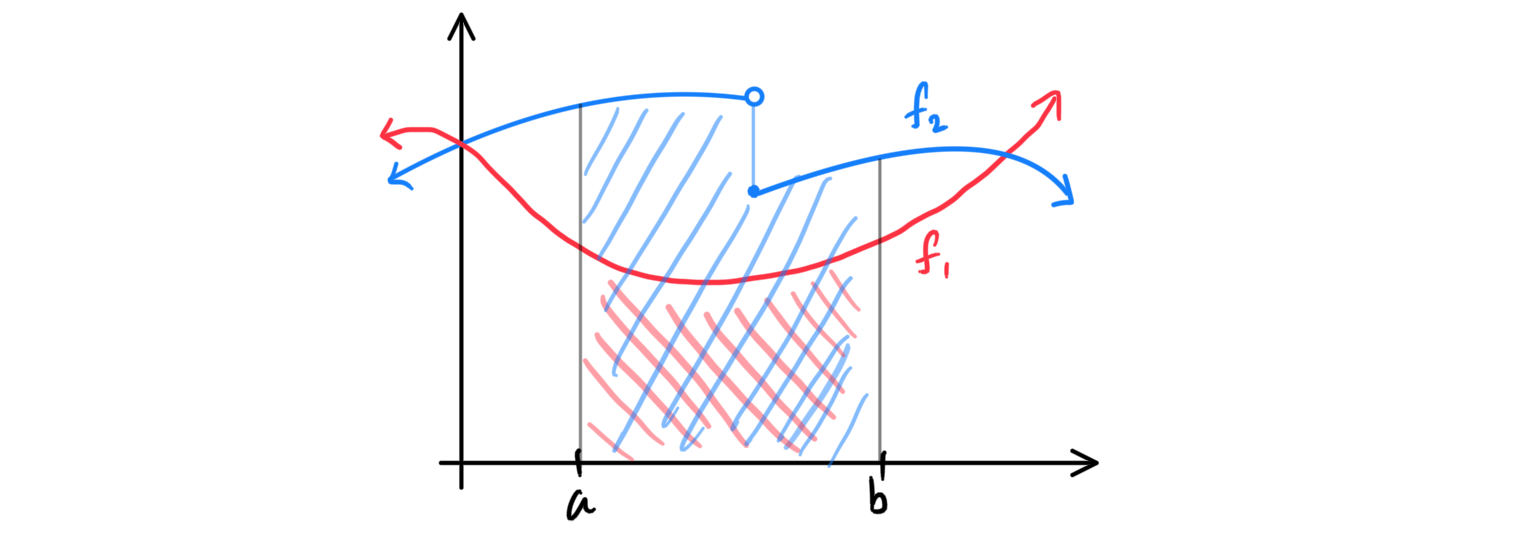
\includegraphics[scale=0.27]{img/Monotonicity_of_Integral.PNG}
      \end{center}
      This immediately implies that given constants $m, M$ such that $m \leq f(x) \leq M$ at each $x \in [a, b]$, we have
      \[m \cdot (b - a) \leq \int_a^b f(x)\,dx \leq M \cdot (b-a)\]
      This is very easily visualized below. 
      \begin{center}
          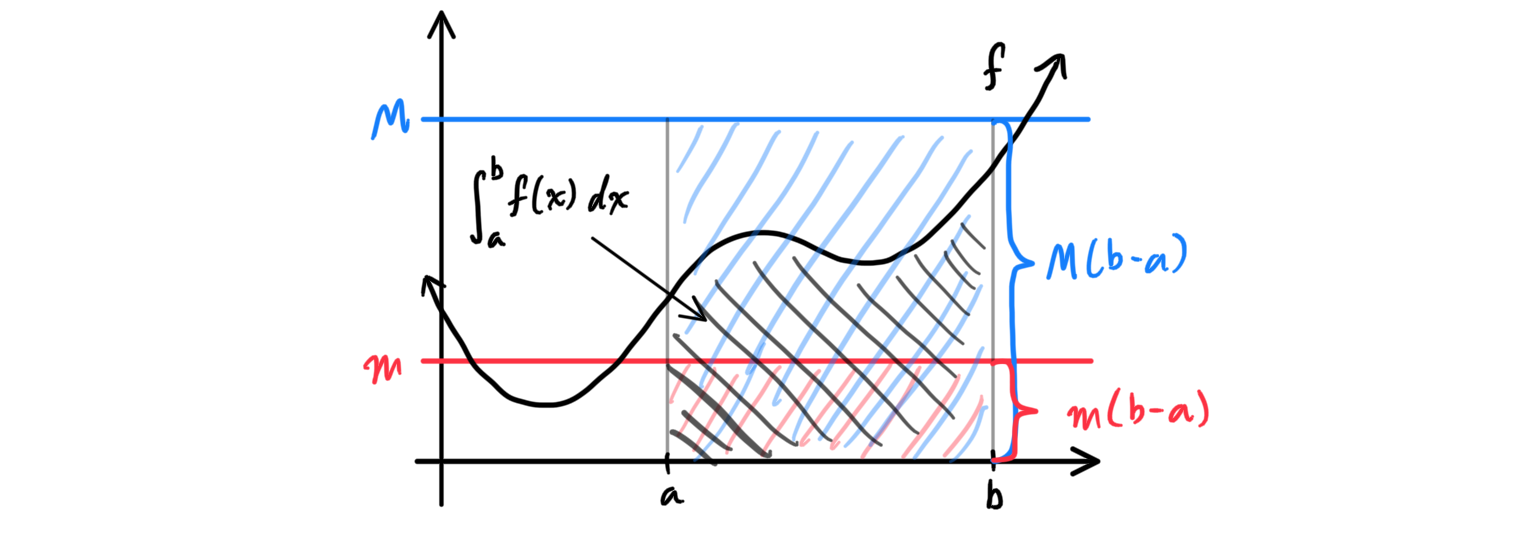
\includegraphics[scale=0.27]{img/Monotonicity_of_Intergral_2.PNG}
      \end{center}
      In particular, if $0 \leq f(x)$ on $[a, b]$, then
      \[0 \leq \int_a^b f(x)\,dx\]
    \end{lemma}

    \begin{theorem}[Mean Value Theorem of the Integral]
    Given $f \in \mathcal{R}[a, b]$, with 
    \[m = \inf_{x \in [a, b]} f(x) \text{ and } M = \sup_{x \in [a, b]} f(x)\]
    then there exists a number $\mu \in [m, M]$ such that
    \[\int_a^b f(x)\,dx = \mu \cdot (b - a)\]
    Furthermore, if $f \in C[a, b]$ (that is, continuous on $[a, b]$), it immediately follows by the intermediate value theorem that there exists a point $\xi \in [a, b]$ such that
    \[\int_a^b f(x)\,dx = f(\xi) (b - a)\]
    \begin{center}
        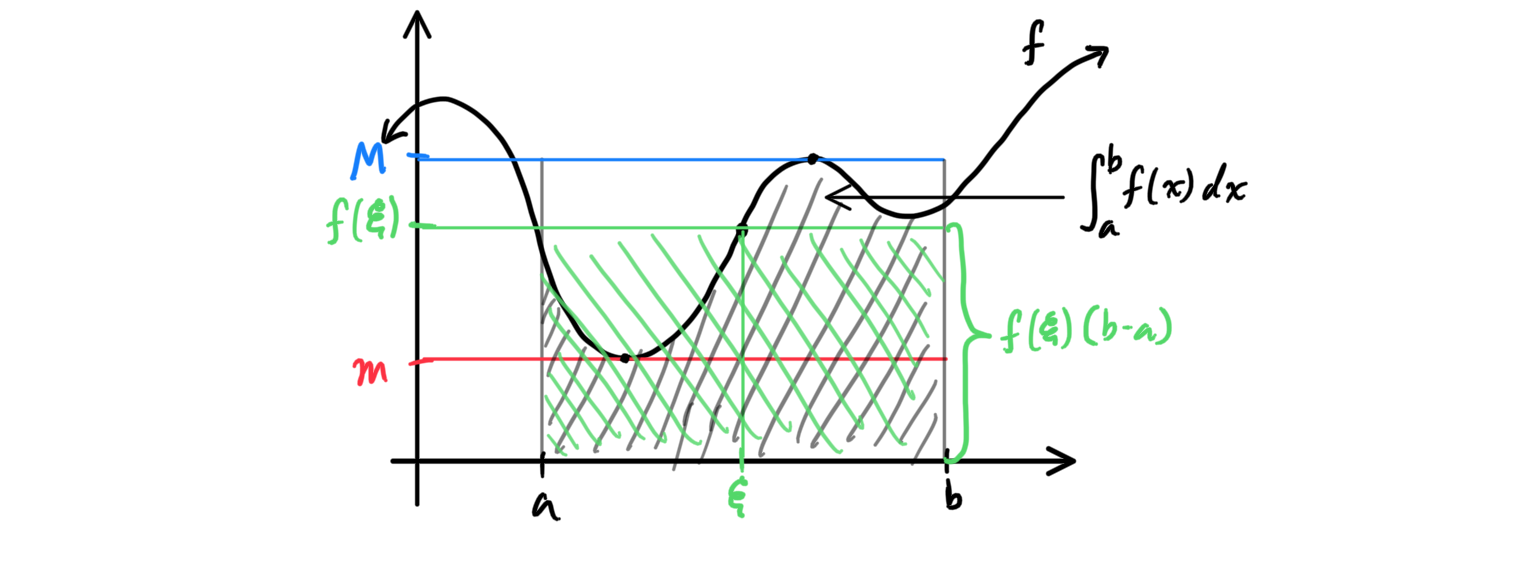
\includegraphics[scale=0.27]{img/Mean_Plus_Intermediate_Value_Theorem_Integral.PNG}
    \end{center}
    \end{theorem}

    Due to the length of the proof, we ask the reader to take it for granted the following theorem. 

    \begin{theorem}[Bonnet's Formula]
    If $f, g \in \mathcal{R}[a, b]$ and $g$ is a monotonic function on $[a, b]$, then there exists a point $\xi \in [a, b]$ such that
    \[\int_a^b (f \cdot g) (x)\,dx = g(a) \int_a^\xi f(x)\,dx + g(b) \int_\xi^b f(x)\,dx\]
    \end{theorem}

  \subsection{Connections between Integrals, Primitives, Derivatives}

    \begin{definition}[Integral with Variable Upper Limit]
      Let $f \in \mathcal{R}[a, b]$, and let us choose an $x \in [a, b]$ in order to construct the function
      \[F(x) \equiv \int_a^x f(t)\,dt\]
      which is called an \textbf{integral with variable upper limit}. Note that since $[a, x] \subset [a, b]$, it follows that $f \big|_{[a,x]} \in \mathcal{R}[a, x]$ and therefore the function $x \mapsto F(x)$ is unambiguously defined for $x \in [a, b]$. 
      \begin{center}
          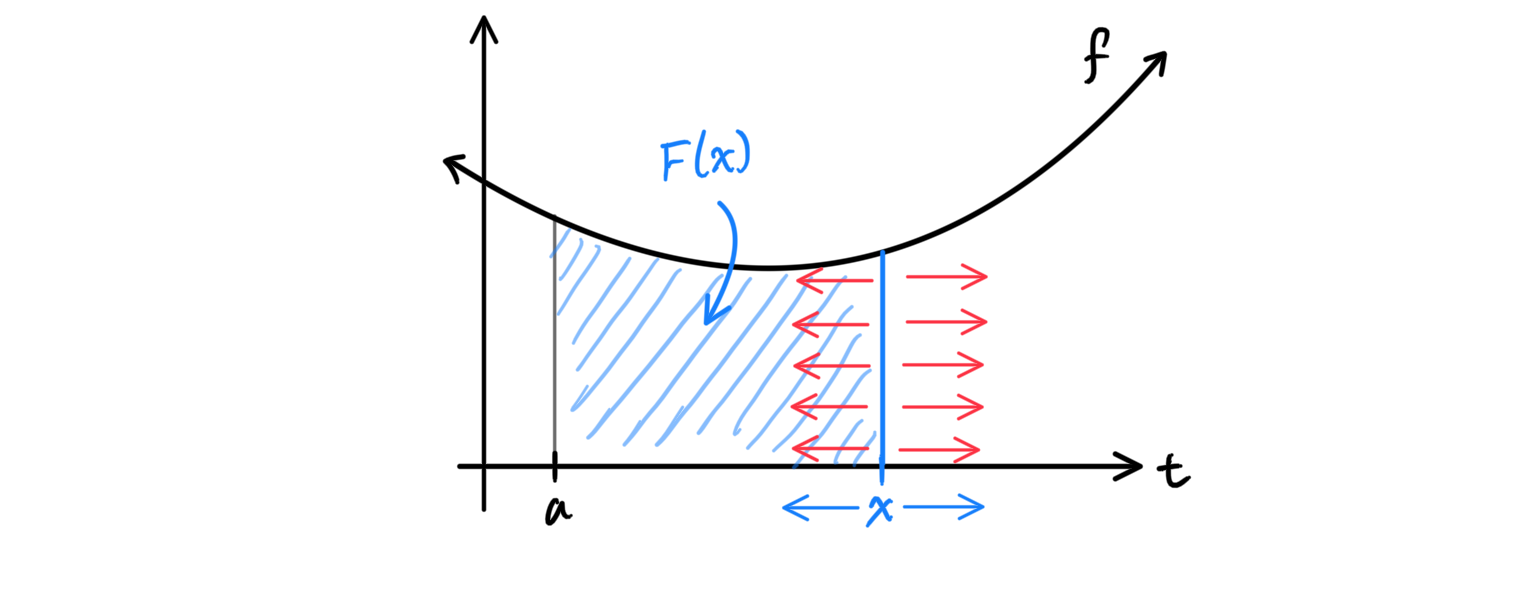
\includegraphics[scale=0.27]{img/Integral_with_Variable_Upper_Limit.PNG}
      \end{center}
      Furthermore, $F(x)$ is continuous on $[a, b]$. Since $f$ is integrable on $[a, b]$, it is bounded by a constant $C$ such that
      \[|f(t)| \leq C \text{ on } [a, b]\]
      It follows from the additive properties of the integral and boundedness theorem that 
      \[|F(x + h) - F(x)| \leq C|h|\]
      if $x, x + h \in [a, b]$, as visualized. This means that for any $\delta$-neighborhood of $F(x)$, we can find an arbitrary small $h$ such that the $C|h|$-neighborhood of $F(x)$ is completely contained in the $\delta$-neighborhood. But by the inequality above, this means that there exists an $\epsilon = h$-neighborhood of $x$ such that its entire image is contained within the $C|h|$-neighborhood, which itself is contained within the $\delta$-neighborhood. This shows that $F$ is continuous. 
    \end{definition}

    \begin{theorem}[First Fundamental Theorem of Calculus]
    Let $f \in \mathcal{R}[a, b]$ be continuous at point $x \in [a, b]$ (resp. continuous on closed interval $[a, b]$). Let $F$ be the function, defined for all $x \in [a, b]$ by 
    \[F(x) \equiv \int_a^x f(t)\,dt\]
    Then, $f$ is continuous and differentiable at $x$ (resp. uniformly continuous on $[a, b]$ and differentiable on $(a, b)$), 
    \[F^\prime (x) = f(x)\]
    at $x$ (resp. for all $x \in [a, b]$). This is an amazing fact, because visually, it tells us that the rate at which the integral $F$ is increasing at $x$ (represented by the increasing area under the curve of $f$) is equal to the value of $f$ at the point $x$ itself! 
    \begin{center}
        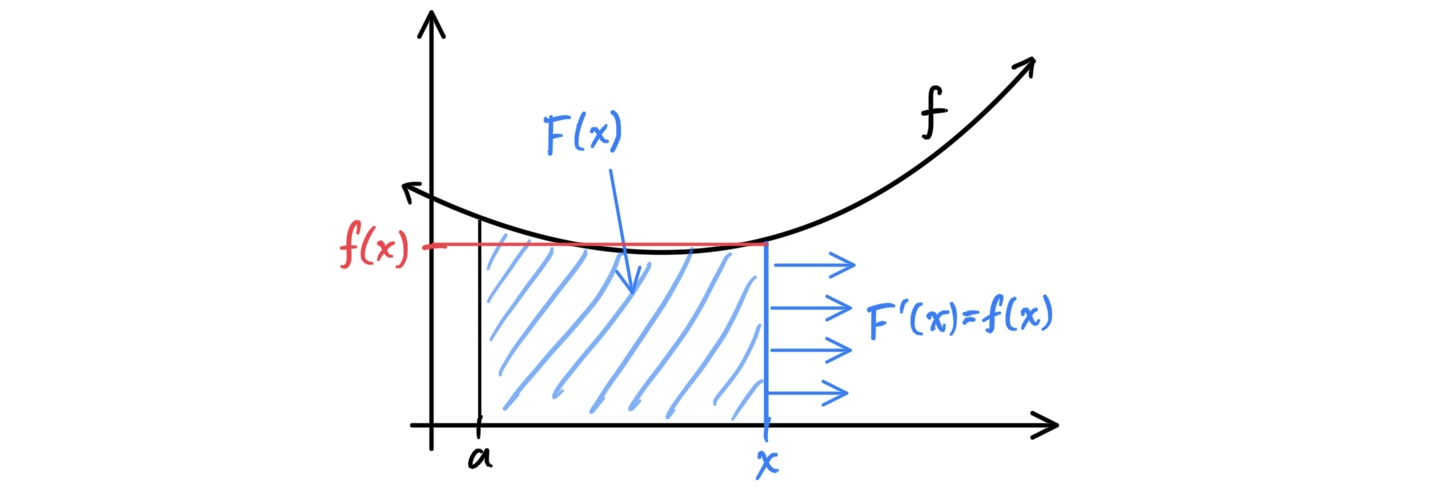
\includegraphics[scale=0.25]{img/First_Fundamental_Theorem_Analysis.jpg}
    \end{center}
    \end{theorem}
    \begin{proof}
    Let $x, x + h \in [a, b]$, and let us estimate the difference $F(x+h) - F(x)$. It follows from the continuity of $f$ at $x$ that $f(t) = f(x) + \Delta(t)$, where $\Delta(t) \rightarrow 0$ as $t \rightarrow x$. If point $x$ is held fixed, the function 
    \[\Delta(t) = f(t) - f(x)\]
    is integrable on $[a, b]$, being the difference of the integrable function $t \mapsto f(t)$ and the constant $f(x)$. Let us denote
    \[M(h) \equiv \sup_{t \in [x, x+h]} |\Delta(t)|\]
    which means that $M(h)$ is the largest difference between $f(x)$ and $f(t)$ in the interval $[x, x+h]$. 
    \begin{center}
        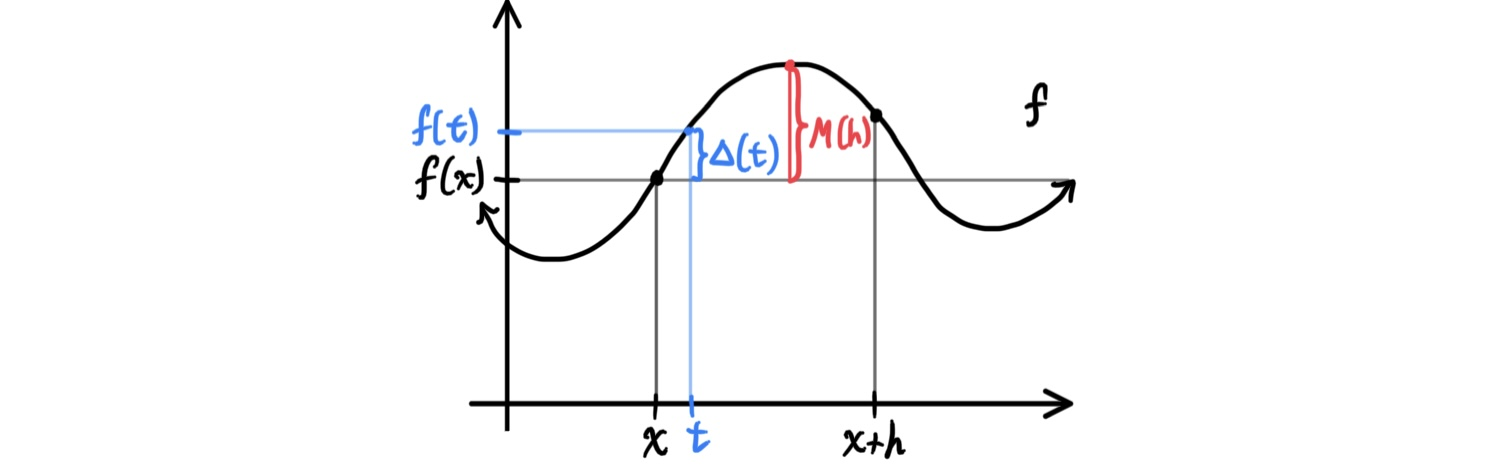
\includegraphics[scale=0.25]{img/Proof_First_Fundamental_Theorem_Analysis.jpg}
    \end{center}
    Clearly $M(h) \rightarrow 0$ as $h \rightarrow 0$. We can now find
    \begin{align*}
        F(x + h) - F(x) & = \int_a^{x+h} f(t)\,dt - \int_a^x f(t)\,dt \\
        & = \int_x^{x+h} f(t)\,dt \\
        & = \int_x^{x+h} \big( f(x) + \Delta(t)\big)\,dt \\
        & = \int_x^{x+h} f(x)\,dt + \int_x^{x+h} \Delta(t)\,dt \\
        & = f(x) h + \alpha(h) h
    \end{align*}
    where we have set 
    \[\int_x^{x+h} \Delta(t)\,dt = \alpha(h) h\]
    where $\alpha$ is infinitesimal as $h \rightarrow 0$, since 
    \[\Bigg| \int_x^{x+h} \Delta(t)\,dt \Bigg| \leq \Bigg| \int_x^{x+h} |\Delta(t)|\,dt \Bigg| \leq \Bigg| \int_x^{x+h} M(h)\,dt \Bigg| = M(h) |h| = \alpha(h)|h|\]
    Therefore, we have shown that if the function $f$ is continuous at a point $x \in [a, b]$, then for displacements $h$ from $x$ such that $x +h \in [a, b]$, the following equality holds.
    \[F(x + h) - F(x) = f(x) h + \alpha(h) h\]
    where $\alpha(h) \rightarrow 0$ as $h \rightarrow 0$, and by definition, this means that $F(x)$ is differentaible on $[a, b]$ at the point $x \in [a, b]$ and that $F^\prime(x) = f(x)$. 
    \end{proof}

    \begin{corollary}
    Every bounded function $f: [a, b] \longrightarrow \mathbb{R}$ on the closed interval $[a, b]$ and has only a finite number of points of discontinuity has a primitive, and every primitive of $f$ on $[a, b]$ has the form 
    \[\mathcal{F}(x) \equiv \int_a^x f(t)\,dt + c\]
    where $c$ is a constant. 
    \end{corollary}

    \begin{theorem}[Second Fundamental Theorem of Calculus]
    Let $f$ be a real-valued function on a closed interval $[a, b]$ with $\mathcal{F}$ any primitive of $f$ on $[a, b]$. If $f$ is Riemann-integrable (i.e. $f$ bounded with finite points of Lebesgue measure zero) on $[a, b]$, then 
    \[\int_a^b f(x)\,dx  = \mathcal{F} \big|_a^b \equiv \mathcal{F}(b) - \mathcal{F}(a)\]
    \begin{center}
        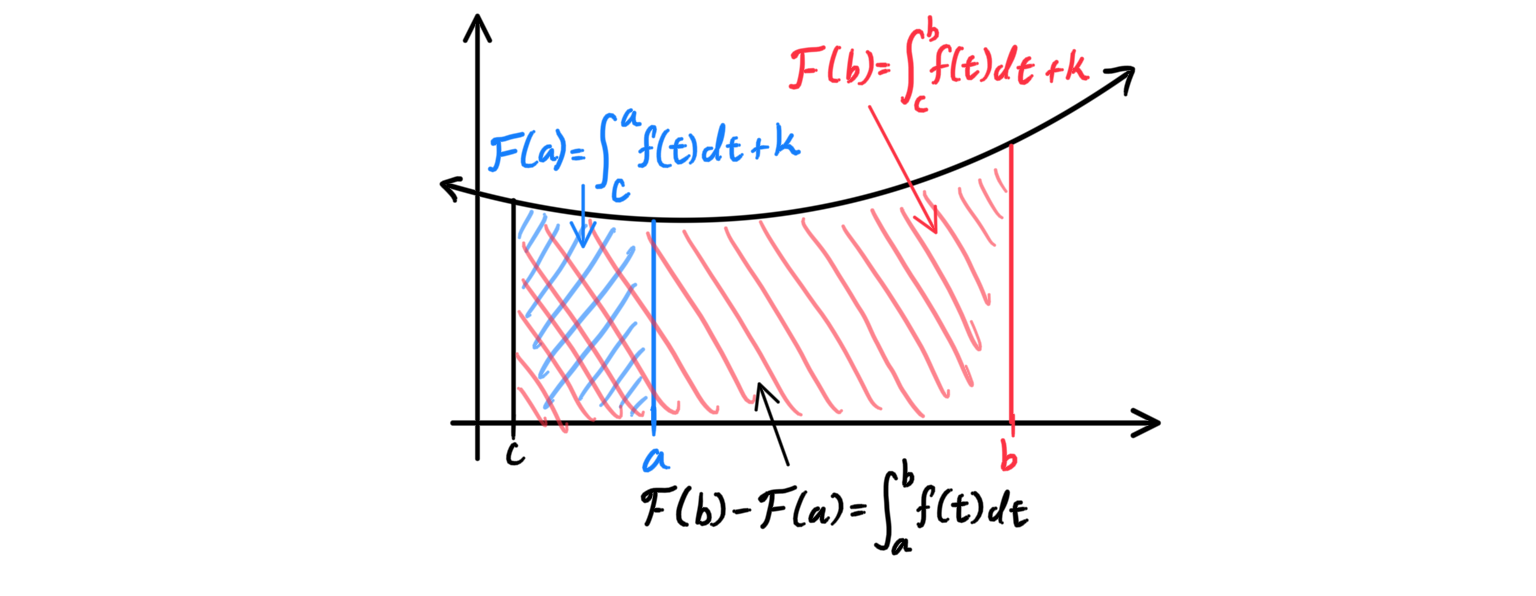
\includegraphics[scale=0.25]{img/Second_Fundamental_Theorem_Analysis.PNG}
    \end{center}
    \end{theorem}
    \begin{proof}
    We already know that a bounded function on a closed interval having a finite number of discontinuities is integrable, and by the corollary, we are guaranteed an existence of a primitive $\mathcal{F}(x)$ of the function $f$ on $[a, b]$ with the form 
    \[\mathcal{F} (x) \equiv \int_a^x f(t)\,dt + c\]
    Setting $x = a$, we find that $c = \mathcal{F}(a)$, and so 
    \[\mathcal{F}(x) \equiv \int_a^x f(t)\,dt + \mathcal{F}(a)\]
    Evaluating $\mathcal{F}$ at $x = b$ gives
    \[\int_a^b f(t)\,dt = \mathcal{F}(b) - \mathcal{F}(a)\]
    \end{proof}

    \subsubsection{Integration by Parts and Taylor's Formula}
    \begin{theorem}[Definite Integration by Parts]
    If the functions $u(x)$ and $v(x)$ are continuously differentiable on a closed interval with endpoints $a$ and $b$, then
    \[\int_a^b (u \cdot v^\prime)(x)\,dx = (u \cdot v)\big|^b_a - \int_a^b (v \cdot u^\prime)(x)\,dx\]
    which is customarily written in the form as
    \[\int_a^b u\,dv = u \cdot v \big|_a^b - \int_a^b v\,du\]
    \end{theorem}
    \begin{proof}
    By the product rule of differentiation, we have
    \[(u \cdot v)^\prime (x) = (u^\prime \cdot v)(x) + (u \cdot v^\prime) (x)\]
    where by hypothesis, $u^\prime \cdot v, u \cdot v^\prime$ are continuous and hence integrable on $[a, b]$. Using the linearity of the integral and the 2nd fundamental theorem of calculus, we get
    \[(u \cdot v) (x) \big|^b_a = \int_a^b (u^\prime \cdot v)(x)\,dx + \int_a^b (u \cdot v^\prime) (x)\,dx\]
    \end{proof}

    \begin{theorem}[Integral Form of the Remainder]
    If $f: E \longrightarrow \mathbb{R}$ has continuous derivatives up to order $n$ on the closed interval $[a, x]$, then Taylor's formula holds
    \[f(x) = f(a) + \frac{f^\prime (a)}{1!} (x - a) + \ldots + \frac{f^{(n-1)}(a)}{(n-1)!} (x - a)^{n-1} + r_{n-1}(a; x)\]
    where 
    \[r_{n-1} (a;x) = \frac{1}{(n-1)!} \int_a^x f^{(n)} (t) (x - t)^{n-1} \,dt\]
    This form is called \textbf{Taylor's formula with the integral form of the remainder}. 
    \end{theorem}
    \begin{proof}
    Using the 2nd fundamental theorem and the definite integration by parts formula, we can carry out the following chain of transformations, assuming continuity and differentiability when needed. 
    \begin{align*}
        f(x) - f(a) & = \int_a^x f^\prime (t) \,dt \\
        & = - \int_a^x f^\prime(t) (x - t)^\prime \,dt \\
        & = -f^\prime (t) (x - t)\big|_a^x + \int_a^x f^{\prime\prime} (t) (x - t) \,dt \\
        & = f^\prime (a) (x - a) - \frac{1}{2} \int_a^x f^{\prime\prime} (t) \big( (x - t)^2\big)^\prime \,dt \\
        & = f^\prime (x - a) - \frac{1}{2} f^{\prime\prime} (t) (x - t)^2 \big|_a^x + \frac{1}{2} \int_a^x f^{\prime\prime\prime} (t) (x - t)^2\,dt \\
        & = f^\prime(a) (x - a) + \frac{1}{2} f^{\prime\prime} (a) (x - a)^2 - \frac{1}{2 \cdot 3} \int_a^x f^{\prime\prime\prime} (t) \big((x - t)^3\big)^\prime\,dt \\
        & = \ldots \\
        & = f^\prime (a) (x - a) + \ldots + \frac{1}{(n-1)!} f^{(n-1)} (a)(x - a)^{n-1} + r_{n-1}(a;x)
    \end{align*}
    where $r_{n-1}(a;x)$ is given by the integral formula mentioned. 
    \end{proof}

    \subsubsection{Change of Variables in Integration}
    We now show and prove the method what we call "u-substitution" for definite integration. 

    \begin{theorem}[Change of Variable]
    If $\varphi: [\alpha, \beta] \longrightarrow [a, b]$ is a continuously differentiable mapping such that $\varphi(\alpha) = a$ and $\varphi(\beta) = b$, then for any continuous function $f(x)$ on $[a, b]$ the function $f\big(\varphi(t)\big) \varphi^\prime (t)$ is continuous on the closed interval $[\alpha, \beta]$ and 
    \[\int_a^b f(x)\,dx = \int_\alpha^\beta f\big(\varphi(t)\big) \varphi^\prime(t)\,dt\]
    \begin{center}
        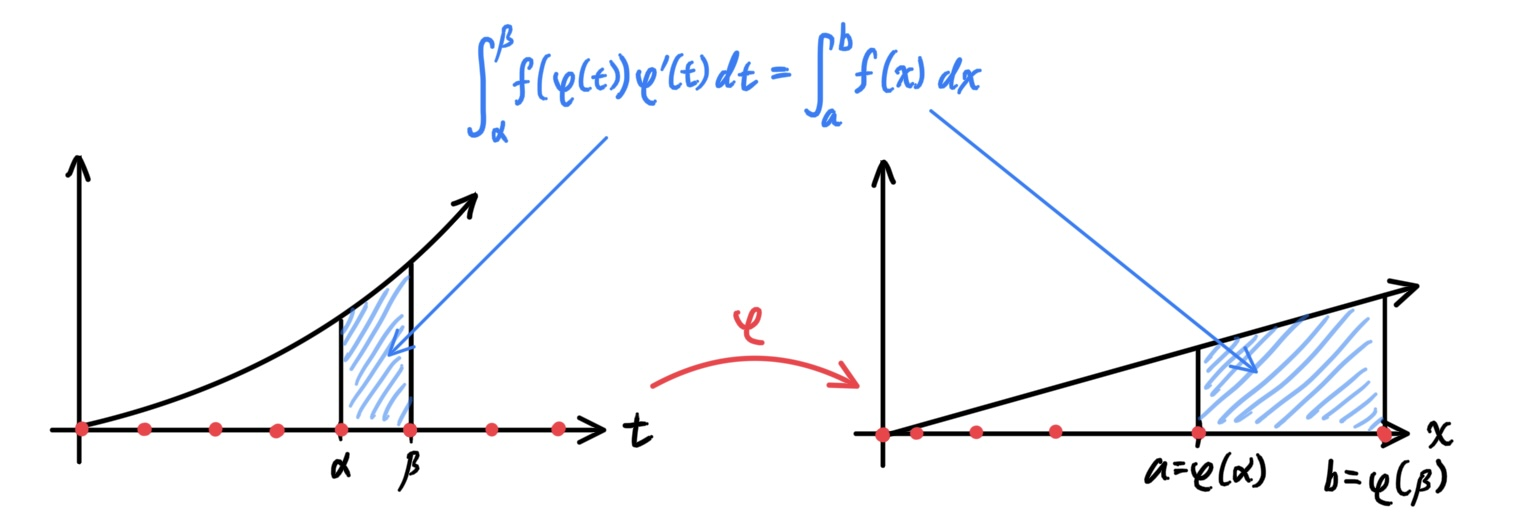
\includegraphics[scale=0.25]{img/Change_of_Variable_Analysis_Integral.jpg}
    \end{center}
    \end{theorem}
    \begin{proof}
    We prove a slightly weaker form of the theorem with the additional hypothesis that $\varphi$ is strictly monotonic. 
    \end{proof}

    \subsubsection{Additive Interval Functions and the Integral}
    In this section we take a step back and construct the integral in a more abstract sense, using the concepts of an additive interval function. 

    \begin{definition}[Additive Interval Function]
      An \textbf{additive (oriented) interval function} is a function 
      \[(\alpha, \beta) \mapsto I(\alpha, \beta) \in \mathbb{R}\]
      that assigns a number $I(\alpha, \beta)$ to each ordered pair of points $(\alpha, \beta)$ of a fixed closed interval $[a, b]$ in such a way that the following equality holds for any triple of points $\alpha, \beta, \gamma \in [a, b]$. 
      \[I(\alpha, \gamma) = I(\alpha, \beta) + I(\beta, \gamma)\]
      Notice that the integral holds this property, shown in the theorem on the symmetric property of the integral. It follows that all additive interval functions are anticommutative: 
      \[I(\alpha, \beta) + I(\beta, \alpha) = 0\]
      which immediately results in
      \[I(\alpha, \alpha) = 0\]
    \end{definition}

    \begin{lemma}[Generating Functions of Additive Interval Functions]
      For any function $x \mapsto \mathcal{F}(x)$ that maps points on the interval $[a, b]$ to $\mathbb{R}$, we set
      \[\mathcal{F}(x) \equiv I(a, x)\]
      and by additivity we have
      \[I(\alpha, \beta) = I(\alpha, \beta) - I(a, \alpha) = \mathcal{F}(\beta) - \mathcal{F}(\alpha)\]
      and thus, every additive oriented interval function has the form 
      \[I(\alpha, \beta) = \mathcal{F}(\beta) - \mathcal{F}(\alpha)\]
      By constructing $I$ in this manner, we say that \textbf{the function $\mathcal{F}$ generates the additive function $I$}. 
    \end{lemma}

    \begin{example}
    If $f \in \mathcal{R}[a, b]$, the function $\mathcal{F} = \int_a^x f(t)\,dt$ generates the additive function
    \[I(\alpha, \beta) = \mathcal{F}(\beta) - \mathcal{F}(\alpha) = \int_a^\beta f(t)\,dt - \int_a^\alpha f(t)\,dt = \int_\alpha^\beta f(t)\,dt\]
    \end{example}

    We conclude by stating a sufficient condition for an additive interval function to be generated by an integral. 
    \begin{theorem}
    Suppose the additive function $I(\alpha, \beta)$ defined for points $\alpha, \beta \in [a, b]$ has the property that, for some known function $f \in \mathcal{R}[a, b]$, 
    \[\inf_{x \in [\alpha, \beta]} f(x) (\beta - \alpha) \leq I(\alpha, \beta) \leq \sup_{x \in [\alpha, \beta]} f(x) (\beta - \alpha)\]
    holds for any closed interval $[\alpha, \beta] \subset [a, b]$ ($\alpha \leq \beta$). Then, the additive function $I$ must be the definite integral
    \[I(a, b) = \int_a^b f(x)\,dx\]
    \end{theorem}

    This theorem is extremely useful. It says that if we have any abstract additive interval function $I(\alpha, \beta)$ that satisfies the properties above, then it \textbf{must} be generated by an integral with variable upper limit, meaning that (by the previous example) $I$ itself must be a definite integral! 

    \subsubsection{Arc Length}
    When modeling systems in physics, one of the most fundamental tools we use are path functions that models the movement of a particle in $\mathbb{R}^3$. 

    \begin{definition}[Path]
      A \textbf{path} in $\mathbb{R}^3$ is a continuous mapping $r: [a, b] \subset \mathbb{R} \longrightarrow \mathbb{R}^3$ defined
      \[t \mapsto \big(x(t), y(t), z(t)\big)\]
      of an interval of the real line into $\mathbb{R}^3$ defined by the (continuous) scalar functions $x, y, z$. The endpoints 
      \[A = \big(x(a), y(a), z(a)\big) \text{ and } B = \big(x(b), y(b), z(b)\big)\]
      in $\mathbb{R}^3$ are called the \textbf{initial point} and \textbf{terminal point} of the path. Furthermore, a path is \textbf{closed} if its initial and terminal points coincide. 
    \end{definition}

    \begin{definition}[Support]
      If $\Gamma: I \longrightarrow \mathbb{R}^3$ is a path, the image $\Gamma(I) \subset \mathbb{R}^3$ is called the \textbf{support} of the path. 
    \end{definition}

    \begin{definition}[Simple Paths]
      A path $\Gamma: I \longrightarrow \mathbb{R}^3$ that is injective is called a \textbf{simple path}, or a \textbf{paramaterized curve}, and its support is called a \textbf{curve} in $\mathbb{R}^3$. 

      A closed path $\Gamma: [a, b] \longrightarrow \mathbb{R}^3$ is called a \textbf{simple closed path/curve} if the path $\Gamma: [a, b) \longrightarrow \mathbb{R}^3$ is simple. 
    \end{definition}

    \begin{definition}[Smooth Paths]
      A path $\Gamma: [a, b] \longrightarrow \mathbb{R}^3$ is $C^k$ smooth if the functions $x(t), y(t), z(t)$ are $C^k$ smooth. $\Gamma$ is \textbf{piecewise smooth} if the closed interval $[a, b]$ can be partitioned into a finite number of closed intervals on each of which the corresponding restriction of $\Gamma$ is smooth. 
    \end{definition}

    Now, we are ready to construct the length of a smooth path $\Gamma: [a, b] \longrightarrow \mathbb{R}^3$. Our initial ideas about the length $l[a, b]$ of the path traversed during the time interval $\alpha \leq t \leq \beta$ are as follows: 
    \begin{enumerate}
      \item If $\alpha < \beta < \gamma$, then $l$ is an additive interval function.
      \[l[\alpha, \gamma] = l[\alpha, \beta] + l[\beta, \gamma]\]
      \item If $v(t) = \big( x^\prime (t), y^\prime (t), z^\prime (t)\big)$ is the velocity of the point at time $t$, then 
      \[\int_{x \in [\alpha, \beta]} |v(t)| (\beta - \alpha) \leq l[\alpha, \beta] \leq \sup_{x \in [\alpha, \beta]} |v(t)| (\beta - \alpha)\]
    \end{enumerate}
    Thus, if the functions $x, y, z$ are continuously differentiable on $[a, b]$, this is sufficient condition (by the theorem in the previous subsection) that the additive function $l$ is an integral.

    \begin{definition}[Arc Length Integral]
      The length of a smooth path $\Gamma: [a, b] \longrightarrow \mathbb{R}^3$ is defined by 
      \[l[a, b] \equiv \int_a^b |\Gamma^\prime (t)|\,dt \equiv \int_a^b \sqrt{x^{\prime 2} (t) + y^{\prime 2} (t) + z^{\prime 2} (t)}\, dt\]
      We can visualize this by partitioning the interval $[a, b]$ into the intervals $\Delta_i$, each with point $\xi_i \in \Delta_i$. This would partition the path to $\Gamma(\Delta_i)$, each with points $\Gamma(\xi_i)$, and at each point $\Gamma(\xi_i)$, we can imagine the velocity vector of the curve. By taking the magnitude of this vector $\Gamma^\prime (\xi_i)$, we multiply it by the length of the interval $\Delta x_i$ to get one rectangle, creating an approximation for one partition of the path. 
      \begin{center}
          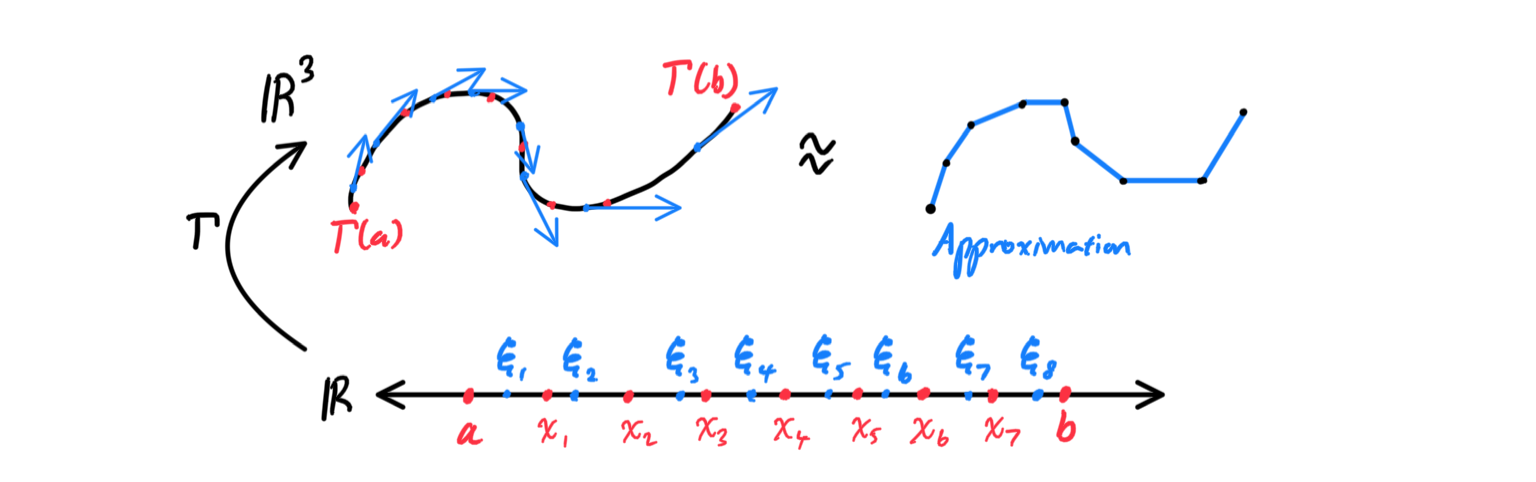
\includegraphics[scale=0.25]{img/Arc_Length_Integral.PNG}
      \end{center}
      An immediate result of this formula is the formula for the length of a graph of a function $f: [a, b] \longrightarrow \mathbb{R}$ in $\mathbb{R}^2$, by looking at the paramaterization $t \mapsto \Gamma(t) = \big(t, f(t)\big)$. 
      \[l[a,b] \equiv \int_a^b \sqrt{1 + (f^\prime (t))^2}\,dt\]
    \end{definition}

    The question on the effect of paramaterization on the integral now arises. 

    \begin{definition}[Admissible Change of Parameter]
      The path $\Tilde{\Gamma}: [\alpha, \beta] \longrightarrow \mathbb{R}^3$ is obtained from $\Gamma: [a, b] \longrightarrow \mathbb{R}^3$ by an \textbf{admissible change of parameter} if there exists a smooth mapping 
      \[T: [\alpha, \beta] \longrightarrow [a, b]\]
      such that $T(\alpha) = a, T(\beta) = b$, $T^\prime (\tau) > 0$ (that is, the reparamaterization $T$ is monotonic) on $[\alpha, \beta]$, and 
      \[\Tilde{\Gamma} = \Gamma \circ T\]
      The series of mappings can be represented with the following commutative diagram, where $I_{\alpha, \beta} = [\alpha, \beta] \subset \mathbb{R}$ and $I_{a, b} = [a, b] \subset \mathbb{R}$. 
      \[
        \begin{tikzcd}
          I_{\alpha, \beta} \arrow{r}{T} \arrow{rd}{\Tilde{\Gamma}}& I_{a, b} \arrow{d}{\Gamma}\\
           & \mathbb{R}^3
        \end{tikzcd}
      \]
      or with the more detailed visual below (Note that the points are labeled $0, 1, 2, 3, 4, 5$ do not represent numerical values, but rather the order in which the points are paramaterized. We can see from this ordering that $T$ is monotonic.)
      \begin{center}
          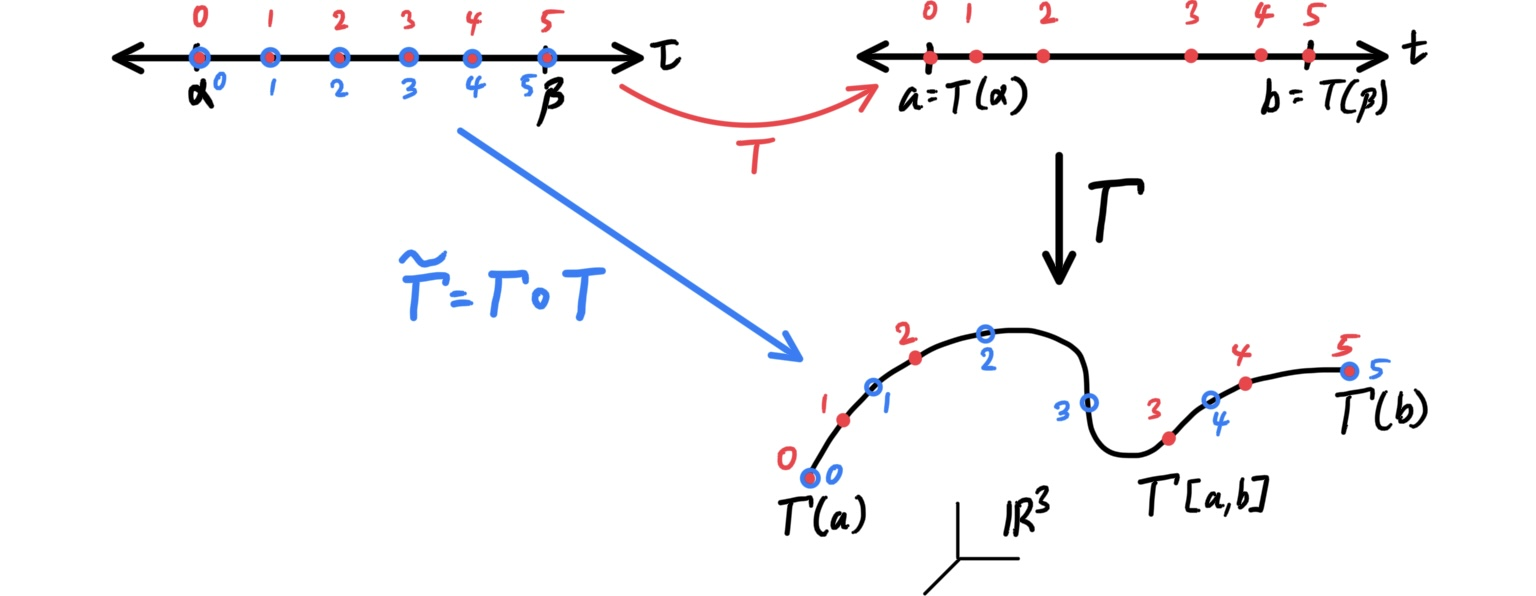
\includegraphics[scale=0.25]{img/Admissible_Change_of_Parameter.jpg}
      \end{center}
    \end{definition}

    \begin{theorem}[Invariance of Arclength Integral under Admissible Change of Parameters]
    If a smooth path $\Tilde{\Gamma}: [\alpha, \beta] \longrightarrow \mathbb{R}^3$ is obtained from a smooth path $\Gamma: [a, b] \longrightarrow \mathbb{R}^3$ by an admissible change of parameter, then the lengths of the two paths are equal. That is, a
    \[\int_a^b |\Gamma^\prime (t) |\,dt = \int_\alpha^\beta |\Tilde{\Gamma}^\prime (t)|\,dt \equiv \int_\alpha^\beta |(\Gamma \circ T)^\prime (t)|\,dt\]
    \end{theorem}

  \subsection{Improper Integrals}

    Due to some limitations of the Riemann integral, we cannot integrate over "singularities" where either the interval or the function is unbounded. We develop the tools of improper integration to deal with this problem; there are two types of improper integrals. 

    \begin{definition}[Improper Integral of Unbounded Interval]
      Suppose the function $x \mapsto f(x)$ is defined on the interval $[a, +\infty)$ and is integrable on every closed interval $[a, b]$ contained in that interval. Then, we call the following term
      \[\int_a^{+\infty} f(x)\,dx \equiv \lim_{b \rightarrow + \infty} \int_a^b f(x)\,dx\]
      the \textbf{improper Riemann integral of $f$ over the interval $[a, +\infty)$} and 
      \[\int_{-\infty}^b f(x)\,dx \equiv \lim_{a \rightarrow -\infty} \int_a^b f(x)\,dx \]
      the \textbf{improper Riemann integral of $f$ over the interval $(-\infty, b]$}.If the limit exists, then we say that the integral \textbf{converges} and \textbf{diverges} otherwise. 
    \end{definition}

    \begin{definition}[Improper Integral of Unbounded Function]
      Suppose the function $x \mapsto f(x)$ is defined on the interval $[a, B)$ and integrable on any closed interval $[a, b] \subset [a, B)$. Then, we call the following term
      \[\int_a^B f(x)\,dx \equiv \lim_{b \rightarrow B^-} \int_a^b f(x)\,dx\]
      the \textbf{improper Riemann integral of $f$ over interval $[a, B)$} and
      \[\int_A^b f(x)\,dx \equiv \lim_{a \rightarrow A^+} \int_a^b f(x)\,dx\]
      the \textbf{improper Riemann integral of $f$ over interval $(A,b]$}.
    \end{definition}

    For cohesiveness, we can combine these two definitions of improper integrals into the following one. 

    \begin{definition}[Improper Integrals]
      Let $[a, \omega)$ be a finite or infinite interval and $x \mapsto f(x)$ a function defined on that interval and integrable over every closed interval $[a, b] \subset [a, \omega)$. Then, by definition
      \[\int_a^\omega f(x)\,dx \equiv \lim_{b \rightarrow \omega} \int_a^b f(x)\,dx\]
      if this limit exists as $b \rightarrow \omega, b \in [a, \omega)$. Similarly, given the finite or infinite interval $(\omega, b]$ with $f$ integrable over every closed interval $[a, b] \subset (\omega, b]$, we have
      \[\int_\omega^b f(x)\,dx \equiv \lim_{a \rightarrow \omega} \int_a^b f(x)\,dx\]
      Note that if $\omega \in \mathbb{R}$ and $f \in \mathcal{R}[a, \omega]$, the improper integral is equivalent to the regular Riemann integral. 
      \[\int_a^\omega f(x) = \lim_{b\rightarrow \omega} \int_a^b f(x)\,dx\]
    \end{definition}

    \begin{lemma}[Properties of the Improper Integral]
      Suppose $f, g$ are functions defined on interval $[a, \omega)$ (without loss of generality, we let $\omega$ be the upper limit of integration) and integrable on every closed interval $[a, b] \subset [a, \omega)$. Suppose the improper integrals 
      \[\int_a^\omega f(x)\,dx \text{ and } \int_a^\omega g(x)\,dx\]
      are well-defined. 
      \begin{enumerate}
        \item For any $\lambda_1, \lambda_2 \in \mathbb{R}$ the function $(\lambda_1 f + \lambda_2 g)(x)$ is integrable in the improper sense on $[a, \omega)$ and
        \[\int_a^\omega (\lambda_1 f + \lambda_2 g)(x)\,dx = \lambda_1 \int_a^\omega f(x)\,dx + \lambda_2 \int_a^\omega g(x)\,dx\]
        \item For any $c \in [a, \omega)$, 
        \[\int_a^\omega f(x)\,dx = \int_a^c f(x)\,dx + \int_c^\omega f(x)\,dx\]
        \item If $\varphi: [\alpha, \gamma) \longrightarrow [a, \omega)$ is a smooth strictly monotonic mapping with $\varphi(\alpha) = a$ and $\varphi(\beta) \rightarrow \omega$ as $\beta \rightarrow \gamma^-$, then the improper integral of the function $t \mapsto (f \circ \varphi)(t) \varphi^\prime (t)$ over $[\alpha, \gamma)$ exists and 
        \[\int_a^\omega f(x)\,dx = \int_\alpha^\gamma (f \circ \varphi)(t) \varphi^\prime (t)\,dt\]
      \end{enumerate}
    \end{lemma}

    \subsubsection{Convergence of an Improper Integral}

      Note that by definition, an improper integral 
      \[\int_a^\omega f(x)\,dx \equiv \lim_{b \rightarrow \omega} \int_a^b f(x) \,dx\]
      is a limit of the function 
      \[\mathcal{F}(b) \equiv \int_a^b f(x)\,dx\]
      as $b \rightarrow \omega$. This means that we can use the Cauchy criterion to determine the convergence of this limit, and hence, existence of this improper integral. 

      \begin{theorem}[Cauchy Criterion for Convergence of an Improper Integral]
      If the function $x \mapsto f(x)$ is defined on the interval $[a, \omega)$ and integrable on every closed interval $[a, b] \subset [a, \omega)$, then the integral 
      \[\int_a^\omega f(x)\,dx\]
      converges if and only if for every $\epsilon > 0$ there exists $B \in [a, \omega)$ such that the relation
      \[\Bigg| \int_{b_1}^{b_2} f(x)\,dx \bigg| < \epsilon\]
      holds for any $b_1, b_2 \in [a, \omega)$ satisfying $B < b_1$ and $B < b_2$. 
      \end{theorem}
      \begin{proof}
      We have
      \[\int_{b_1}^{b_2} f(x)\,dx = \int_a^{b_2} f(x)\,dx - \int_a^{b_1} f(x)\,dx = \mathcal{F}(b_2) - \mathcal{F}(b_1)\]
      and therefore the condition is simply the Cauchy criterion for the existence of a limit for the function $\mathcal{F}(b)$ as $b \rightarrow \omega$. 
      \end{proof}

      \begin{definition}[Absolute Convergence of an Improper Integral]
        The improper integral 
        \[\int_a^\omega f(x)\,dx\]
        \textbf{converges absolutely} if the integral
        \[\int_a^\omega |f|(x)\,dx\]
        converges. Clearly, the inequality
        \[\Bigg| \int_{b_1}^{b_2} f(x)\,dx \Bigg| \leq \Bigg| \int_{b_1}^{b_2} |f|(x)\,dx \Bigg|\]
        implies that if an improper integral converges absolutely, then it converges. 
      \end{definition}

      This study of absolute convergence reduces to the study of convergence of integrals of nonnegative functions. The following lemma is useful in determining convergence of such functions. 

      \begin{lemma}
        Let there be a function $f$ defined on interval $[a, \omega)$ that is also integrable over every closed interval $[a, b] \subset [a, \omega)$. If $f(x) \geq 0$ on $[a, \omega)$, then the improper integral 
        \[\int_a^\omega f(x)\,dx\]
        exists if and only if the function 
        \[\mathcal{F}(b) \equiv \int_a^b f(x)\,dx\]
        is bounded on $[a, \omega)$. 
      \end{lemma}
      \begin{proof}
      It is clear that 
      \[\int_a^\omega f(x)\,dx = \lim_{b \rightarrow \omega} \mathcal{F}(b)\]
      If $f(x)\geq 0$, then the function $\mathcal{F}(b)$ is nondecreasing on $[a, \omega)$ and therefore has a limit as $b \rightarrow \omega$ only if it is bounded (since every monotonically increasing sequence that is bounded always converges). 
      \end{proof}

      This leads to the familiar integral test for convergence of a series. 

      \begin{theorem}[Integral Test for Convergence of a Series]
      If the function $x \mapsto f(x)$ is defined on the interval $[1, +\infty)$, nonnegative, nonincreasing, and integrable on each closed interval $[1, b] \subset [1, +\infty)$, then the series 
      \[\sum_{n=1}^\infty f(n) = f(1) + f(2) + \ldots\]
      and the integral 
      \[\int_a^{+\infty} f(x)\,dx\]
      either both converge or both diverge. 
      \end{theorem}

      We can use the comparison test analogue to determine convergence of improper integrals. 

      \begin{theorem}[Comparison Test for Convergence of Improper Integrals]
      Suppose the functions $f(x), g(x)$ are defined on the interval $[a, \omega)$ and integrable on any closed interval $[a, b] \subset [a, \omega)$. If 
      \[0 \leq f(x) \leq g(x)\]
      on $[a, \omega)$, then 
      \[\int_a^\omega g(x)\,dx \text{ converges} \implies \int_a^\omega f(x)\,dx \text{ converges}\]
      and the inequality 
      \[\int_a^\omega f(x)\,dx \leq \int_a^\omega g(x)\,dx\]
      holds. Also, 
      \[\int_a^\omega f(x)\,dx \text{ diverges} \implies \int_a^\omega g(x)\,dx \text{ diverges}\]
      \end{theorem}
    
    \subsubsection{Improper Integrals with Multiple Singularities}

      \begin{definition}[Improper Integral with Both Limits as Singularities]
        Given singularities $\omega_1, \omega_2$, the improper integral is defined
        \[\int_{\omega_1}^{\omega_2} f(x)\,dx \equiv \int_{\omega_1}^c f(x)\,dx + \int_c^{\omega_2} f(x)\,dx\]
        where $c$ is an arbitrary point in $(\omega_1, \omega_2)$. 
      \end{definition}

    \begin{example}[Gaussian Integral]
    The integral 
    \[\int_{-\infty}^{+\infty} e^{-x^2}\,dx = \sqrt{\pi}\]
    \end{example}

